%!TEX program = xelatex
\documentclass[a4paper,12pt,openany,twoside]{book} % twoside
\usepackage[inner=3.5cm,outer=2.5cm, top=2.5cm]{geometry} %showframe

\usepackage{url}
\usepackage{fontspec}
\usepackage{lmodern}
\usepackage{csquotes}
\usepackage{graphicx}
\usepackage{caption}
\usepackage{subcaption}
\usepackage[rgb]{xcolor}
\graphicspath{ {assets/} }
\usepackage{xunicode}
\usepackage{xltxtra}
\usepackage{chngcntr}
\usepackage[czech]{babel}
\usepackage[pagestyles,medium]{titlesec}
\usepackage{setspace}
\usepackage{emptypage}
\usepackage{xpatch}
\usepackage{caption}
\usepackage{subcaption}
\usepackage{ragged2e}
\usepackage{pbox}
\usepackage{rotating}
\usepackage{float}
\usepackage{afterpage}
\usepackage{tipa}
\usepackage{array}
\usepackage{wrapfig}
\usepackage{multirow}
\usepackage{tabularx}
\usepackage{booktabs}
\newcolumntype{C}{>{\centering\arraybackslash}X}
\usepackage{lscape}
\usepackage{bashful}

\usepackage[hidelinks]{hyperref}

\usepackage{mdframed}
\usepackage{framed}
\def\tightlist{}

\xpatchcmd{\part}{\thispagestyle{plain}}{\thispagestyle{empty}}{}{}


\newcommand\exmp{\textsf}

\counterwithout{figure}{chapter}
\counterwithout{footnote}{chapter}


\newpagestyle{sensible}{
	\headrule\sethead{}{}{\MakeUppercase{\chaptertitle}}
	\setfoot{}{\thepage}{}
}

\setlength\emergencystretch{1em}
\setlength\headheight{14pt}
\setstretch{1.1}
\setcounter{secnumdepth}{4}

\widowpenalty10000
\clubpenalty10000

\hyphenation{выпа-дений}

\setmainfont[Ligatures=TeX]{CMU Serif Roman}

\usepackage[backend=biber, style=iso-authoryear, sortlocale=cs\_CZ, uniquelist=false, autocite=footnote, maxcitenames=2, maxbibnames=99, minnames=1, urldate=long, spacecolon=false,bibencoding=UTF8
]{biblatex}
\let\oldmultinamedelim\multinamedelim
\let\oldfinalnamedelim\finalnamedelim
\renewcommand*{\multinamedelim}{~a~}
\renewcommand*{\finalnamedelim}{~a~}
\renewcommand*{\nameyeardelim}{~}
\AtBeginBibliography{%
  \renewcommand*{\multinamedelim}{~--\space}%
  \renewcommand*{\finalnamedelim}{~--\space}%
}
\DefineBibliographyStrings{czech}{%
  mathesis = {Bakalářská diplomová práce},
  editors = {eds.}
}

\addbibresource{bibliography.bib}

\newcommand{\sign}[1]{%      
  \begin{tabular}[t]{@{}r@{}}
  \makebox[2.5in]{\dotfill}\\
  \strut#1\strut
  \end{tabular}%
}


\begin{document}
	\clearpage
	\pagenumbering{gobble}

	\begin{titlepage}
		\begin{center}
			{\Large\uppercase{Masarykova univerzita}}

			\vspace{1em}

			{\Large Filozofická fakulta}

			\vspace{1em}

			{\large Ústav českého jazyka}

			\vspace{1em}

			{\large Počítačová lingvistika}

			\vspace{11em}

			{\large Kryštof Davídek }
			
			\vspace{3em}
			
			{\LARGE\bf Webová aplikace pro geografické zmapování krajanských komunit a jejich jazyka}

			\vspace{3em}

			{\Large Magisterská diplomová práce}

			\vfill
			\vspace{3em}
			Vedoucí práce: PhDr. Marie Kopřivová, Ph.D.
			
			2022
		\end{center}
	\end{titlepage}


\cleardoublepage

\par
\par\vspace*{\fill}
	\pagestyle{plain}
\pagenumbering{roman}
\begin{flushright}
	Prohlašuji, že jsem magisterskou diplomovou práci vypracoval samostatně s~využitím uvedených pramenů a~literatury.

	\vspace{3em}

	    \makebox[2.5in][r]{\dotfill}
	    
	    Kryštof Davídek

	    \par

\end{flushright}
\clearpage

\par
\par\vspace*{\fill}

Na tomto místě bych rád poděkoval své vedoucí práce doktorce Marie Kopřivové za veškeré rady a~poznatky, které mi ochotně poskytovala po celou dobu psaní této práce.

\clearpage

\section*{Abstrakt}

Předkládaná diplomová práce si klade za cíl navrhnout a~vytvořit na základě dostupných údajů mapu krajanské češtiny, která zahrnuje komunity českých krajanů rozšířených po světě. Mapa krajanské češtiny má podobu interaktivní webové aplikace, která také obsahuje uživatelsky přívětivou administraci pro vkládání nových historických, jazykových a~geografických dat týkajících se jednotlivých komunit. V~aplikaci je v~tuto chvíli zpřístupněno několik modelových příkladů, které vychází ze zpracovaných materiálů. Vývoj uživatelského rozhraní probíhal v~javaScriptové knihovně React a~pro persistenci dat byla zvolena platforma Firebase.

\section*{Abstract}

The aim of this thesis is to design and develop a~geographical mapping of compatriot communities and their language around the world based on available data. The map takes the form of an interactive web application, which also includes a~user-friendly administration for entering new historical, linguistic and geographical data concerning individual communities. Several model examples are currently available in the application, based on the materials developed. The user interface development was done in the React JavaScript library and the Firebase platform was chosen for data persistence.

\section*{Klíčová slova}

Krajanská čeština, krajané, webová aplikace, mapa krajanské češtiny, React

\section*{Keywords}

Compatriot Czech, compatriots, web application, geographical mapping of compatriot language, React

\clearpage

\tableofcontents


\cleardoublepage
\pagenumbering{gobble}

% \newgeometry{top=2.5cm}

\pagenumbering{arabic}
\hypertarget{uxfavod}{%
\chapter*{Úvod}\label{uvod}\addcontentsline{toc}{chapter}{Úvod}}

Současný odhad počtu lidí žijících mimo území České republiky, kteří se hlásí k~českému původu, je 2--2,5 milionů~\parencite{Krajane-mv2}. Velké množství českých krajanů pochází z~historicky formovaných krajanských komunit, jež jsou často unikátní, díky své specifické kombinaci tehdejší české kultury a~určitých zahraničních vlivů.

V~dnešní době sice existuje řada projektů, které se snaží zachytit současný stav krajanských komunit ve světě, často jde však pouze o~částečná řešení, jež primárně odkazují na existující krajanské spolky.

Cílem této diplomové práce je tak navrhnout a~implementovat na základě dostupných údajů mapu krajanské češtiny, která zahrnuje komunity krajanů rozšířených po světě. Výsledná webová aplikace se skládá z~vizualizace geografického rozšíření komunit a~administračního prostředí pro přidávání transkriptů, zvukových nahrávek a~doprovodných informací pro jednotlivé krajanské oblasti.

Práce se skládá ze dvou částí -- teoretické a~praktické. V~teoretické části nejprve představujeme základní pojmosloví vztahující se k~problematice českých krajanů a~věnujeme se tématu českého vystěhovalectví. Zde popisujeme vývoj emigrací na českém území od poloviny 16. století po konec 20. století. Na závěr této kapitoly charakterizujeme termíny spojené s~tématem enklávy českého jazyka.

Druhou kapitolou teoretické části je popis několika význačných krajanských komunit ve světě, u~nichž lze reflektovat asimilační vývoj jazyka, a~jsou tak dobrými ukázkami využití aplikace v~praxi.

V~praktické části popisujeme celkový vývoj výsledné webové aplikace. Nejprve představujeme několik souvisejících projektů, jimiž jsme se při tvorbě částečně inspirovali, a~zaměřujeme se na analýzu funkčních a~nefunkčních požadavků.

Dále se věnujeme návrhové části, kde uvádíme použité technologie, charakterizujeme strukturu a~obsah dat a~na konkrétních obrazovkách z~aplikace popisujeme uživatelské rozhraní s~nejdůležitějšími interakčními prvky. Závěrečná kapitola se věnuje implementačním detailům na vybraných příkladech kódu.

\part{Teoretická část}

\hypertarget{ux10deskuxe9-vystux11bhovalectvuxed}{%
\chapter{České vystěhovalectví}\label{ux10deskuxe9-vystux11bhovalectvuxed}}

Ústředním tématem této magisterské diplomové práce jsou komunity českých krajanů v~Evropě a~ve světě. V~první kapitole si proto nejprve představíme základní pojmosloví vztahující se k~této problematice a~popíšeme si vývoj českého vystěhovalectví, který je důležitý pro pochopení vzniku českých diaspor ve světě. V~závěru kapitoly se v~krátkosti zaměříme na téma enklávy českého jazyka a~jazykových ostrovů, které tuto látku rozšiřují o~lingvistický kontext.

Tato obecnější část tak poslouží jednak jako pevný teoretický základ pro charakteristiku významnějších komunit českých krajanů, tak i~pro popis některých částí návrhu a~implementace webové aplikace v~praktické části této diplomové práce.

\hypertarget{krajanstvuxed}{%
\section{Krajanství}\label{krajanstvuxed}}

I~přes to, že se s~pojmem \emph{krajan} v~literatuře zabývající se problematikou emigrace pracuje jako se zavedeným termínem, neexistuje pro něj zcela jednoznačná definice. V~širším pojetí (ať už jde o~kontext politický, odborný či publicistický) se lze sice setkat s~významem \uv{osoby žijící dočasně či trvale mimo území České republiky, které se hlásí k~českému národu či k~českému původu}, nicméně tato obecná definice začíná být problematická v~okamžiku, kdy se začneme detailněji zabývat jednotlivými aspekty krajanství\footnote{Otázky, jež tuto definici problematizují, mohou znít ku příkladu tímto způsobem: \uv{Lze  za českého krajana považovat člověka hlásícího se k~českému národu, nebo je zapotřebí vlastnit dokumenty svědčící o~daném původu?} anebo \uv{Musí se tito lidé organizovat do izolovaných enkláv či krajanských spolků, nebo mohou žít nezávisle na zavedených institucí?}~\parencite{Jakoubek2015}.}~\parencite{Jakoubek2015}.

Ze sociologického hlediska je význam tohoto pojmu nejčastěji úmyslně či neúmyslně zaměňován s~českými výrazy jako jsou \emph{emigrant}, \emph{zahraniční Čech}, \emph{vystěhovalec}, \emph{exulant} apod., nicméně se převážně jedná o~nesjednocené a~často libovolně zaměnitelné pojmy. Resp. u~slov \emph{krajan} a~\emph{emigrant} (\emph{vystěhovalec)} si lze v~českém kontextu všimnout na konci minulého století mírného významového posunu. Někteří političtí českoslovenští vystěhovalci, kteří emigrovali po roce 1948 a~1968 po sametové revoluci v~roce 1989 o~sobě prohlásili, že se již nepovažují za emigranty tehdejšího Československa, nýbrž za české či slovenské krajany -- pominul tak totiž důvod ke klasifikaci vystěhovalců založené na právním či politickém vztahu k~dané zemi~\parencite{Broucek2017}.

Můžeme tak vyvodit, že pojem \emph{krajan} částečně souvisí se subjektivním vnímáním postavení každého z~konkrétních jedinců a~že je tato identifikace spíše dynamickým procesem\footnote{Vliv na tento proces má více faktorů, jako jsou například diasporizace (sounáležitost krajanů s~mateřskou zemí), vliv národního státu, transnacionalizace (přeshraniční vazby krajanů) a~míra integrace krajana v~dané zemí~\parencite{Broucek2017}.}, který lze těžko přesně definovat jednou objektivní definicí.

Obecnější význam tohoto výrazu zastávají i~další autoři, kteří vnímají synonymní vztah s~pojmem \emph{příslušník českého národu}, u~nějž je primárně artikulován etnický rozměr. Tento přístup ale podléhá určité kritice, jelikož implicitně vynucuje odmítnutí sounáležitosti s~jiným etnikem~\parencite{Jakoubek2015}. Jak bylo výše zmíněno, vnímání \emph{krajanství} záleží na perspektivě jedinců či skupin žijících v~zahraničí a~jejich začlenění do dané etnické skupiny.

Každopádně i~přes všechny problematické aspekty ohledně jednoho obecného významu popsaných výše se v~České republice pro administrativní účely za krajana považuje \uv{každý cizinec, který má prokazatelně český národnostní původ, nebo je dítětem rodiče s~českým národnostním původem, nebo dítětem dítěte rodiče s~českým národnostním původem}~\parencite{Krajane-mv1}.

Současný odhad počtu lidí žijících mimo území ČR, kteří se hlásí k~českému původu, je 2--2,5 milionů~\parencite{Krajane-mv2}, a~jelikož byly historicky příčiny české emigrace spíše důsledkem perzekuce a~jiných tlaků~\parencite{Vaculik2009a}, snaží se Česká republika krátce po svém osamostatnění krajanské komunity různými způsoby podporovat. Zpočátku byly nejčastější formou pomoci rozličné rozvojové projekty -- tento model podpory byl ale později vystřídán systémem finanční podpory prostřednictvím Ministerstva zahraničních věcí (dále MZV)~\parencite{Broucek2009}.

Tyto záležitosti v~MZV spravoval samostatný odbor krajanských a~nevládních styků (později odbor kulturních a~krajanských vztahů) a~v~současné době se jim věnuje Pracoviště pro krajanské záležitosti v~čele se zvláštním zmocněncem pro krajanské záležitostí. Tohle pracoviště se již nevěnuje pouze poskytování peněžních darů na kulturní projekty, nýbrž zajišťuje vzdělávací programy (jako jsou například kurzy českého jazyka), zajišťuje vydávání potvrzení o~příslušnosti k~české krajanské komunitě v~zahraničí, anebo informuje o~již existujících krajanských spolcích~\parencite{Krajane-mv3}.

Obecným cílem všech těchto aktivit je podpořit kulturní dědictví, které se s~jednotlivými krajanskými komunitami pojí. Nicméně záměrem není pouze udržovat nebo vytvářet určitou formu \emph{skanzenů}, nýbrž aktivně podporovat interakce zahraničních a~domácích Čechů, kteří se tímto způsobem vzájemně obohacují~\parencite{Broucek2009}.

Konkrétní projekty zabývající se podporou krajanských komunit, které jsou nějakým způsobem relevantní pro naši praktickou část, popisujeme v~kapitole \ref{souvisejuxedcuxed-projekty}.

\hypertarget{migrace}{%
\section{Migrace}\label{migrace}}

Hlavní příčinou pro vznik zahraničních krajanských komunit jsou procesy spojené s~jevem migrace (za české synonymum se pro tento pojem považuje výraz \emph{stěhování}). Jde o~mezinárodní pohyby větších skupin obyvatelstva, vedoucí k~setrvání (i)migrantů v~hostitelské zemi alespoň po určitou dobu (v~současné době se za tuto dobu podle Organizace spojených národů považuje minimálně jeden rok). Tyto procesy lze chápat jako protikladné vůči přirozenému, biologicky podmíněnému pohybu obyvatelstva, přičemž nezáleží na typu a~síle příčin, které migrační pohyb vyvolaly~\parencite{Nespor2005}.

Tuto problematiku lze studovat ze dvou možných pohledů v~závislosti na směru migračního pohybu z~hlediska dané země, kterou migrant opouští (emigrace, česky vystěhovalectví), případně kam směřuje (imigrace, česky přistěhovalectví)~\parencite{Fialova2017b}. Další důležitým pojmem je reemigrace -- návrat části emigrantů (případně jejich potomků) do jejich země původu\footnote{Příkladem může být státem organizované reemigrace po 2. světové válce do pohraničních oblastí anebo po revoluce 1989 z~černobylské oblasti Ukrajiny a~Běloruska~\parencite{Vaculik2002}.}~\parencite{Nespor2005}.

Pokud se ale migranti po prvotní, tedy primární migraci rozhodnou přesunout do další země, jako se například vydala část banátských Čechů do Bulharska na přelomu 19. a~20. století, jedná se pak o~sekundární migraci. Při opakovaných migračních pohybech v~rámci dvou stejných oblastí (s~tím že jedna z~nich je země původu) tento proces nazýváme transmigrací\footnote{Jedná se například o~migrační systém současných ukrajinských pracovníků v~České republice~\parencite{Nespor2005}.}~\parencite{Nespor2005}.

Jev transmigrace začal být ve vědecké obci více reflektován na konci 20. století, a~to hlavně z~důvodu masové migrace způsobené globalizací, kdy jsou zahraniční migranti díky novým technologiím neustále v~kontaktu se svojí zemí původu. Pro akademické potřeby tak vznikl koncept \emph{transnacionální migrace}, jenž se zaměřuje na proces, při němž imigranti vytváří a~udržují vzájemné sociální vazby se společností původní země~\parencite{Kralova2013}. Jak je z~definice patrné, tento přístup je spíše aplikovatelný na migrační systémy 20.--21. století., nicméně lze některá z~jeho východisek aplikovat i~na historický vývoj některých krajanských komunit.

Také je zapotřebí dodat, že proces migrace ovlivňuje skladbu obyvatelstva obou lokalit (zvláštně pokud se jedná o~hromadné, ne-li organizované přesuny) a~následné změny významně působí nejen na strukturu místní populace, ale i~na předpoklady jejího dalšího vývoje. Proto historicky existovaly snahy tyto procesy přímo nebo nepřímo regulovat, a~to ať už částečným nebo úplným zákazem vystěhování či přistěhování obyvatelstva. Typickým důsledkem těchto opatření bývá nelegální imigrace, jíž se snaží na globální úrovni řešit na zvláštní orgánu při OSN (Vysoký komisař OSN pro uprchlíky), nicméně i~tak má mnoho hospodářsky vyspělých zemí vlastní migrační politiku, prostřednictvím které se snaží masovou imigraci určitým způsobem ovlivňovat~\parencite{Fialova2017a}.

\hypertarget{historickuxfd-vuxfdvoj-ux10deskuxe9-emigrace}{%
\section{Historický vývoj české emigrace}\label{historickuxfd-vuxfdvoj-ux10deskuxe9-emigrace}}

Migrace obyvatelstva, které pocházelo z~českého území, má dlouhou historii sahající až do 16. století. Jelikož v~průběhu doby existovaly různé příčiny (náboženské, hospodářské a~politické) české emigrace a~reemigrace, lze tohle téma rozdělit do tří částí\footnote{Každopádně důvody pro emigraci nebyly vždy pouze jedné konkrétní povahy, ale vzájemně se ovlivňovaly. Například náboženská emigrace často souvisela se sociálními a~politickými aspekty dané doby~\parencite{Vaculik2009a}.}. Každá z~nich mapuje odlišné období a~popisuje tak hlavní charakteristiky vzniku jednotlivých krajanských komunit.

\hypertarget{nuxe1boux17eenskuxe1-emigrace}{%
\subsection{Náboženská emigrace}\label{nuxe1boux17eenskuxe1-emigrace}}

Za první hromadný odliv Čechů za hranice se považuje českobratrská emigrace do Polska po porážce stavovského odboje v~roce 1547, kdy dal Ferdinand I. Habsburský příslušníkům Jednoty bratrské na vybranou, a~to buď konvertovat k~utrakvismu, anebo emigrovat~\parencite{Vaculik2009a}.

Druhou zaznamenanou události, která způsobila významné vystěhování českého obyvatelstva, byla bitva na Bílé hoře v~roce 1620. V~prvních třech desetiletí po porážce českých stavů odešlo několik tisíc šlechtických a~měšťanských rodin se strachu před perzekucemi a~tresty za účast v~českém stavovském povstání. Tito převážně evangeličtí vystěhovalci odcházeli nejčastěji do německých evangelických státu, hlavně do Saska a~Braniborska. Menší množství exulantů pak zůstalo ve Slezsku či v~Uhrách, kde nebyl vliv Habsburků tak omezující. U~těchto skupin došlo k~úspěšně asimilaci\footnote{Asimilací v~sociologickém kontextu myslíme proces, prostřednictvím kterého se migrující, často minoritní skupina stává součástí skupiny majoritní a~dochází tak k~integraci kulturních znaků z~jednoho kulturního systému do druhého~\parencite{Petrusek2017}.} s~původním obyvatelstvem a~po méně než dvou až tří generací volně splynuly s~daným prostředím~\parencite{Vaculik2002}.

Slezsko, respektive jeho pruská část, dále nabylo na významnosti v~letech 1713--1756, kdy z~důvodu vypuknutí slezských válek mezi Pruskem a~Rakouskem došlo k~větší migrační vlně způsobené především náboženskými agitacemi ze strany tehdejšího Pruského království. Za tuto dobu kolonizovalo do tehdy zpustošené oblasti pruského Slezska až 900 tisíc českých emigrantů, jimž byl dán volný prostor k~vytvoření zemědělských osad a~hlavně svoboda protestanského vyznání~\parencite{Vaculik2002}.

Jak je z~předchozích kapitol patrné, exulanti se primárně zabývali agrární činností, jelikož byla v~pozadí náboženského tlaku částečně i~motivace spojená se zemědělskou kolonizací~\parencite{Broucek2017}.

V~roce 1793 nastává druhé dělení Polska, jež iniciuje další emigrační vlnu protestanských Čechu z~Pruského Slezska. Zde je již problematické hovořit o~čistě náboženské emigraci, protože se zde objevují důvody spojené s~hledáním lepších životních podmínek. Původní emigranti směřuji do více směrů -- protestantského Německa (Střelínsko, Opolsko), katolického Polska (Táborsko, Zelovsko), ale později i~do tehdejšího Ruska, konkrétně Volyňské gubernie (zde se připojili k~již existující vystěhovalecké skupině z~českých zemí) nebo Chersonské a~Tauridské oblasti~\parencite{Vaculik2009a}.

Poslední zmíněnou, nábožensky motivovanou, emigrací je vystěhování východo-českých sektářů do oblasti dnešního rumunského Banátu na přelomu 18. a~19. století. Důvodem tohoto nuceného vystěhování byla snaha habsburské monarchie přesunout vůdce nekatolíků do vzdálených oblastí, které hraničily s~tehdejší Osmanskou říší a~kde byla náboženská pluralita tolerována~\parencite{Nespor2005}. Takto vznikla například osada Svatá Helena, o~níž společně s~ostatními banátskými vesnicemi píšeme v~kapitole \ref{banuxe1t}.

\hypertarget{hospoduxe1ux159skuxe1-emigrace}{%
\subsection{Hospodářská emigrace}\label{hospoduxe1ux159skuxe1-emigrace}}

O~sociálněekonomické nebo také hospodářské emigraci lze uvažovat v~období 19. a~první poloviny 20. století a~týkala se především obyvatelstva v~produktivním věku napříč sociálními vrstvami. Tehdejší habsburská monarchie zpočátku vystěhovalectví nijak výrazně neomezovala, nicméně v~roce 1851 došlo k~úpravě předpisu o~vystěhovalectví, kvůli čemuž nastalo několik významných emigračních vln. Hlavní destinací na počátku 50. let 19. století byly pro obyvatelstvo ze západních Čech Spojené státy americké, které primárně řemeslníky lákaly svým hospodářským potenciálem. Naopak emigranti z~východní části směřovali spíše do rakouských oblastí Balkánu, tedy do již zmíněného Banátu, Srbska, Slavonska nebo Chorvatska~\parencite{Vaculik2009b}.

Kromě USA vystěhovalci směřovali přes hranice Rakouska-Uherska také do nově vzniklého Bulharska, do Polska a~do Volyňské gubernie tehdejšího Ruska, tedy do dnešního Běloruska, Polska a~Ukrajiny. Celkově šlo o~několik desítek tisíc osob, které vytvořily etnicky trvající české enklávy a~jež splynuly s~dosavadními krajanskými komunitami v~těchto oblastech (například již zmíněný Banát nebo Polsko, kam se krajané už dříve přesídlili)~\parencite{Nespor2005}.

Hlavním důvodem českého vystěhovalectví v~této době byla neutěšená ekonomická situace a~s~ní spojené špatné sociální podmínky. Tuto základní motivaci často podporovala organizovaná agitace zahraničních společností profitujících z~masové přepravy emigrantů (např. německé dopravní firmy zajišťující lodní přepravu do Ameriky) a~také zvací dopisy od již vystěhovaných Čechů, které se tiskly do mnohých časopiseckých článků~\parencite{Vaculik2009a}.

Proti těmto proemigračním náladám musel v~druhé půlce 19. století zakročit rakouský stát, protože přestávalo jít o~nepatrný odliv obyvatelstva, nýbrž o~nenávratnou ztrátu pracující a~vojenské síly. Proto začaly vznikat takzvané \uv{povolenky k~trvalému vystěhování}, po jejichž získání ztratil vystěhovalec rakouské občanství\footnote{Tohle opatření mělo být prevencí k~návratu neúspěšných, a~tedy chudých emigrantů zpátky do státu – byly tak vydávány pouze finančně zaopatřeným obyvatelům~\parencite{Vaculik2002}.}. Vláda se dále snažila ovlivňovat veřejné mínění protivystěhovaleckou propagandou (jak pomocí tisku, tak výukou na školách), prostřednictvím které rozšiřovala neúspěšné příběhy emigrantů ze zahraniční a~snažila se tak odradit další občany k~cestě. V~rámci této propagandy byla obyvatelstvu také doporučována vnitřní kolonizace do málo zalidněných Uher, kde byly rozsáhlé volné zemědělské oblasti vlastněné tehdejším Rakouskem (konkrétně šlo o~Sedmihradskou župu Brassó). Této možnosti využilo menší množství vystěhovalců, primárně chudších poměrů, jež si nemohli dovolit cestu do Ameriky~\parencite{Vaculik2009b}.

Na přelomu 19. a~20. století došlo na českém území habsburské monarchie k~částečnému přelidnění obyvatelstva, jež vedlo k~dalším vlnám vystěhovalectví do Německa (na úkor Vídně) a~do USA, kde byly mzdy vyšší a~půda levnější. Nicméně rozhodující byly i~další důvody jako například náboženská svoboda, zbavení se branné povinnosti v~rakousko-uherské armádě či útěk před politickými tresty. Už v~této době době začaly vznikat první krajanské spolky pod hlavičkou zahraničního odboru Národní rady české, který se zabýval osvětovou činností a~šířením české kultury v~zahraničních krajanských komunitách (šlo primárně o~německé lokality jako Vestfálsko, Lipsko nebo Drážďany)~\parencite{Vaculik2009b}.

Po vzniku samostatné Československé republiky došlo k~první snaze realizovat státem organizovanou reemigrační politiku, jejímž cílem byl systematický přesun zahraničních Čechů zpátky do nově vzniklé republiky. Tento pokus, motivován budovatelskými záměry, nakonec nebyl realizován -- a~to jednak z~důvodu chybějících finančních prostředků, tak převážně nezájmu českých menšin z~vyspělejších západních státu jako bylo např. USA\footnote{Organizovaná reemigrace se ale přeci jen u~pár krajanských komunit zdařila, například přesun někdejších náboženských vystěhovalců z~polského Zelówa~\parencite{Nespor2005}.}\footnote{I přes to, že se někteří vystěhovalci státní organizované pomoci nedočkali, podnikali reemigraci na vlastí náklady. Odhaduje se, že se po vzniku První republiky do vlasti navrátilo 200 tisíc lidí~\parencite{Vaculik2009b}.}. Československý stát tak české zahraniční komunity podporoval alespoň prostřednictvím Československého ústavu zahraničního, jehož úkolem bylo mimo jiné zajišťovat činnost krajanských spolků ve světě~\parencite{Nespor2005}.

I~přes to, že po první světové válce USA zavedlo maximální kvóty pro evropské emigranty, české vystěhovalectví se ve dvacátých až třicátých letech 20. století zcela nezastavilo. Emigrovalo menší množství lidí (odhaduje se na 40 tisíc ročně) a~mířili především do zámořské Argentiny a~Kanady spolu s~evropskou Francií, Rakouskem a~Německem. Pohyb obyvatelstva navíc nebyl omezován právem, protože v~roce 1922 vyšel v~platnost vystěhovalecký zákon, který nijak nelimitoval svobody týkající se možností vystěhování ze země~\parencite{Vaculik2009b}.

\hypertarget{politickuxe1-emigrace}{%
\subsection{Politická emigrace}\label{politickuxe1-emigrace}}

Politická emigrace v~českých zemí se týká převážně období po roce 1938, resp. za její počátek lze uvést podepsání Mnichovské dohody a~pozdější začátek okupace nacistickým vojskem. Bezprostředně po odevzdání českého pohraničí Německu vznikla první emigrační vlna na západ do Francie, Velké Británie a~Ameriky (v~menší míře i~do tehdejší SSSR) tvořená hlavně obyvatelstvem, které se obávalo potenciálního pronásledování německým režimem (případně chtěli proti aktuálnímu vývoji v~Československu bojovat ze zahraničí). Typickými vystěhovalci tak byli židé (kvůli obavám z~rasové perzekuce), českoslovenští politici, žurnalisté a~důstojníci\footnote{Masová emigrace však začala 15. března 1939, kdy byly obavy z~války bezprostřednější a~začaly vznikat organizované sítě na převádění uprchlíků do Polska a~tehdejší Jugoslávie~\parencite{Vaculik2002}.}~\parencite{Nespor2005}.

Po skončení druhé světové války reemigrovala zpátky do Československa jen určitá část vystěhovalců\footnote{Např. valná část válečných emigrantů se nevrátila zpátky do země, protože viděli hrozbu ve vzrůstající komunistické moci~\parencite{Vaculik2009a}}. Stát primárně podporoval osídlení pohraničních oblastí, které byly v~tuto chvíli vyprázdněné od Němců -- tuto výzvu vyslyšeli hlavně krajané z~jihoevropských a~východoevropských zemí. Přistěhování se týkalo především potomků zahraničních exulantů, nicméně i~tak některé oblasti po této migrační vlně téměř zanikly (např. severobulharské Vojvodovo)~\parencite{Nespor2005}.

Dalším milníkem byl komunistický převrat v~roce 1948, na nějž česká společnost reagovala různými způsoby, emigrací nevyjímaje. Jen do roku 1953 odešlo z~ČSR na 44 tisíc osob, z~nichž byla naprostá většina (až 88 procent) bez stranické příslušnosti, a~znovu se tak jednalo o~lidí, kteří se báli politické perzekuce, případně se chtěli podílet na zahraničním protikomunistickém odboji~\parencite{Vaculik2002}. Na podporu těchto vystěhovalců vznikaly za pomoci vlád západních států různé instituce. Šlo například o~Radu svobodného Československa, Společnost pro vědy a~umění a~další projekty rozhlasového vysílání anebo tisku~\parencite{Nespor2005}.

Tato skupina českých exulantů byla značně posílena po invazi sovětských vojsk v~roce 1968, jež nastala jako reakce na krátkodobý úpadek represivních složek a~mechanismů českého komunistického režimu a~celkového společenského uvolnění\footnote{Důsledkem politického uvolnění v~období Pražského jara docházelo k~četným zahraničním reemigracím převážně z~Jugoslávie, Bulharska a~Rumunska~\parencite{Nespor2005}.}. Migrační vlna na počet osob předčila poúnorovou emigraci (šlo celkově o~přibližně dvěstě tisíc osob, směřujících primárně do západní Evropy, USA, Austrálie, Kanady, ale i~třeba do Jihoafrické republiky) a~i~díky západním sdělovacím prostředkům se stala velmi významnou ve světě~\parencite{Vaculik2002}.

Každopádně je již problematické tvrdit, že se jednalo o~výhradně politicky motivované emigrace, jelikož se příčiny vystěhování mnohdy mísily s~hospodářskými důvody~\parencite{Broucek2017}.

Po pádu komunistických režimů ve střední a~východní evropě docházelo především k~reemigracím (opět lze těžko tvrdit, že se jednalo pouze o~politicky motivované pohyby, znovu byly spíše hospodářského charakteru) zpátky do České republiky u~zejména mladších generací krajanských komunit. Celkově šlo přibližně o~10 procent všech emigrovaných obyvatel. Je zapotřebí dodat, že ne všechny návraty probíhaly bez komplikací, například v~Rumunsku přistěhovalcům tamější orgány často nevycházely vstříc a~návrat do vlasti značně komplikovaly~\parencite{Nespor2005}.

Na začátku 90. let tak v~zahraničí žilo přibližně 2 až 3 miliony lidí\footnote{Odhaduje se, že začátkem 90. let žilo v~USA 1,5 milonů Čechů a~Slováků, v~Německu a~Rakousku 70 tisíc a~ve Francii 30 tisíc. Na desetitisíce se dají odhadovat počty Čechů a~Slováků též v~Maďarsku, Jugoslávii, Polsku, Rumunsku, Kanadě, v~zemích bývalého SSSR a~v~Argentině~\parencite{Broucek2017}.}, jež do určité míry vnímali svoji českou národnost. Část z~nich (hlavně Češi usídlení v~průmyslových oblastech) se do velké míry asimilovala\footnote{Faktory, na kterých závisí úroveň asimilace, jsou např. velikost skupiny, kompaktnost osídlení, subjektivní důvody a~objektivní příčiny k~vystěhování, míra odlišností prostředí mezi emigrační a~imigrační zemí a~četnost a~kvalita kontaktů s~českými zeměmi~\parencite{Petrusek2017}.} s~odlišnou etnicitou, avšak potomci zemědělských exulantů z~18. a~19. století, kteří se vystěhovali do zemí východní a~jihovýchodní Evropy, si obvykle některé prvky české etnicity, a~tedy i~kultury včetně českého jazyka, úspěšně zachovaly~\parencite{Broucek2017}.

\hypertarget{enkluxe1va-ux10deskuxe9ho-jazyka}{%
\section{Enkláva českého jazyka}\label{enkluxe1va-ux10deskuxe9ho-jazyka}}

Z~jazykovědné perspektivy lze na zahraniční krajanské komunity nahlížet jako na kompaktní seskupení českého obyvatelstva mimo území českého národního jazyka, jež vznikaly typicky dvěma možnými způsoby. Jednak mohlo být dříve území, kde se komunita aktuálně vyskytuje, součástí české jazykové oblasti (například staré české osídlení v~polském Kladsku), anebo se tyto lokality vyskytují mimo souvislou oblast českého jazyka vytvořené prostřednictvím migračních pohybu (jde tedy o~příklady, které jsme uváděly v~předchozích podkapitolách).

Tyto lokality nazýváme \emph{jazykové ostrovy} a~jejich hlavním znakem je souvislé navázání k~určité české nářeční oblasti podle okolností vzniků konkrétní komunity a~současně začlenění do jiného státního celku. Díky izolovanosti enkláv lze tak do velké míry studovat problematiku českých dialektů, protože je u~těchto komunit dochovaná velká mírá nářečních prvků~\parencite{enklava2017}.

\hypertarget{vuxfdznamnuxe9-krajanskuxe9-komunity-ve-svux11btux11b}{%
\chapter{Významné krajanské komunity ve světě}\label{vuxfdznamnuxe9-krajanskuxe9-komunity-ve-svux11btux11b}}

V~následující kapitole si představíme několik význačných krajanských komunit ve světě, jejichž historický vývoj a~aktuální stav je již literaturou alespoň do jisté míry popsán. Jedná se tedy o~takové jazykové enklávy, u~nichž lze významněji reflektovat asimilační vývoj jazyka a~jsou tak dobrými ukázkami využití naší webové aplikace v~praxi. V~rozsahu této diplomové práce každopádně není vložit všechny informace vypsané níže do digitálního formátu, ale spíše vybrat určité části (ať už jednotlivé osady nebo celé lokality), které demonstrují možnosti a~funkce vytvořené webové aplikace viz XXX.

\hypertarget{banuxe1t}{%
\section{Banát}\label{banuxe1t}}

\hypertarget{historickuxfd-vuxfdvoj}{%
\subsection*{Historický vývoj}\label{historickuxfd-vuxfdvoj}}

Rumunský Banát se nachází na jihozápadě Rumunska a~do roku 1552 byl součástí uherské říše, než byl dobyt Turky. Po vyhnání tureckých sil v~roce 1718 se z~oblasti stala zpustošená krajina, jejíž jižní část zůstala z~velké části neobydlena. Právě tohle území se stalo pro české emigranty cílovou destinací, jelikož nabízelo zlepšení tehdejších životních podmínek. Kolonizátorům byla od majitele pozemků nabídnuta půda, dřevo na stavbu domů spolu s~nářadím a~dalšími nutnostmi k~založení osad~\parencite{Secka1995}.

Do Banátu se první čeští vystěhovalci dostali v~letech 1820--1821. Šlo přibližně o~80 rodin, jež byly tvořeny převážně drobnými řemeslníky, zemědělci, ale i~vysloužilími vojáky. Byly to především obyvatelé z~Plzeňska, Domažlicka, Klatovska, Kladenská a~Čáslavská a~založili na rumunském území dvě osady -- Elisabethfeld a~Svatou Helenu (Češi katolického původu se usídlili do Elisabethfeldu, evangeličtí emigranti pak založili druhou zmíněnou osadu)~\parencite{Gecse2013}.

Zpočátku byl pro české exulanty pobyt na novém území velmi náročný. Potřebovali se vypořádat s~odlišnými přírodními podmínkami, jako byl kopcovitý terén a~nepřístupné lesy, ale i~kruté zimy či nebezpečná divoká zvířata. Problémem též byly počáteční neshody s~nájemníkem pozemků, jež se měl o~vystěhovalce starat, nicméně v~roce 1826 i~s~majetkem odjel a~nechal kolonisty napospas. I~tak se podařilo díky začlenění do tehdejší Vojenské hranice kolonie založit a~vytvořit tak podhoubí pro další migrační pohyby na území Banátu~\parencite{Secka1995}.

Druhá emigrační vlna se konala v~letech 1826--1828. Ta již byla pod správou rakouských vojenských úřadů, protože vojenská správa byla spokojena se zapojením emigrantů do Vojenské hranice a~chtěla tak navýšit stavy na strategickém území hranice habsburského státu. Tato nabídka se setkala se zájmem, jelikož v~tu dobu probíhala na českém území hospodářská krize -- tuto výzvu proto vyslyšelo přes 1800 rodin~\parencite{Frnochova2012}.

Vystěhovalcům byla na náklady státu zajištěna lodní doprava po Dunaji (na rozdíl od první vlny, kdy se krajané stěhovali prostřednictvím vozů) a~kolonizovali místa, jež byla vybrána vojenskými úřady. Vznikly tak nové osady Bígr, Eibenthál, Rovensko, Šumice a~Gerník, které byly ale vzájemně kvůli nedostupnému terénu do značné míry izolovány a~vznikaly tak uzavřené komunity. S~okolním obyvatelstvem (Rumuny a~Srby) se tedy emigranti příliš nestýkali a~s~úřady Vojenské hranice komunikovali výlučně německy, i~proto se české národní povědomí krajanů v~těchto komunitách úspěšně drží~\parencite{Secka1995}.

Po zrušení Vojenské hranice v~roce 1871 se Banát stal součástí Uherského státu, důsledkem této události bylo časté nahrazování češtiny jakožto školního jazyka za maďarštinu (z~důvodu dosazování maďarských učitelů do škol). Nicméně například v~katolické Svaté Heleně byla zřízena samostatná škola, kde se stále vyučovalo českým jazykem, nikoliv státním maďarským jazykem~\parencite{Gecse2013}.

V~období první světové války bojovali někteří muži z~Českého Banátu nejčastěji na italské a~ruské frontě, každopádně i~přes to, že byly české vesnice na krátkou dobu obsazeny Srbskými jednotkami, nebyl život v~komunitách výrazněji ovlivněn~\parencite{Gecse2013}.

Větší odliv emigrantů způsobila až druhá světová válka, po níž reemigrovala zpátky na české území až třetina Čechů. Důvodem byla jak situace v~tehdejším Československu (kvůli velké ztrátě obyvatel stát apeloval na přesídlení krajanů zpět do vlasti), tak neutěšený stav v~samotných krajanských osadách (v~průběhu doby došlo k~nedostatku půdy a~v~důsledku přelidnění i~k~šíření různých chorob)~\parencite{Secka1995}.

Díky těžko přístupnému terénu a~nepříliš úrodné půdě byly české osady do velké míry izolovány i~za komunistického režimu, jenž plnil politiku kontrolovaného hospodářství. Vesnice sice platily daně, ale vyhnuly se větším perzekucím ze strany státu~\parencite{Frnochova2012}.

Český jazyk se nadále v~komunitách udržel, protože po roce 1945 do Rumunska přicházeli učitele z~Československa. Dokonce byla v~roce 1972 v~nedalekém městě Nadlaku otevřena přípravka pro budoucí slovenské a~české učitele, kteří už v~roce 1976 nastupovali do škol v~jednotlivých vesnicích. Dalším činitelem, který významně přispěl k~zachování českého jazyka a~české kultury obecně, byly pravidelné duchovní akce v~nedělní škole, díky kterým se i~mladá generace učila české kultuře a~historii~\parencite{Vaculik2009b}.

Po roce 1989 se o~etnické menšiny v~celém rumunském Banátu začaly víc zabývat jejich mateřské země, Československo a~pozdější České republika nevyjímaje. Český zastupitelský úřad v~Bukurešti často za spolupráce rumunských úřadů realizoval systematickou podporu vesnic formou humanitární pomoci (od roku 1995 začal tuto činnost koordinovat nadace Člověk v~tísní). Snahou tak bylo stabilizovat českou populaci v~jižním Banátu, nicméně demografický vývoj českých vesnic má do dnešního dne spíše klesající tendenci viz srov. populace u~jednotlivých českých vesnic za roky 1991 a~2009.

\begin{table}[h!]
\centering
\begin{tabular}{||l c c||}
\hline
Česká vesnice & 1991 & 2009 \\ [0.5ex]
\hline\hline
Svatá Helena & 800 & 357 \\
\hline
Gernik & 910 & 340 \\
\hline
Rovensko & 235 & 205 \\
\hline
Bígr & 360 & 218 \\
\hline
Šumice & 205 & 104 \\ [1ex]
\hline
Eibenthal (a~Ujbánye) & 3110 & 1525 \\ [1ex]
\hline
\end{tabular}
\caption{Demografický vývoj českých vesnic v~Banátu za roky 1991–2009}
\label{table:1}
\end{table}

\hypertarget{jazyk}{%
\subsection*{Jazyk}\label{jazyk}}

\hypertarget{volyux148}{%
\section{Volyň}\label{volyux148}}

\hypertarget{historickuxfd-vuxfdvoj-1}{%
\subsection*{Historický vývoj}\label{historickuxfd-vuxfdvoj-1}}

\hypertarget{jazyk-1}{%
\subsection*{Jazyk}\label{jazyk-1}}

\hypertarget{kavkaz}{%
\section{Kavkaz}\label{kavkaz}}

\hypertarget{texas}{%
\section{Texas}\label{texas}}

\part{Praktická část}

\hypertarget{analuxfdza-poux17eadavkux16f-na-aplikaci}{%
\chapter{Analýza požadavků na aplikaci}\label{analuxfdza-poux17eadavkux16f-na-aplikaci}}

V~praktické části této diplomové práce popisujeme výslednou webovou aplikaci\footnote{Výsledná aplikace je v~tuto chvíli plně funkční pod URL adresou https://czech-map.netlify.app.} pro geografické zmapování krajanských komunit a~jejich jazyka (dále jen aplikace). V~následujících kapitolách si ve stručnosti popíšeme související projekty, z~nichž jsme se při tvorbě inspirovali. Dále aplikaci představíme jak z~pohledu funkčních a~nefunkčních požadavků, tak z~hlediska návrhových a~implementačních částí.

\hypertarget{souvisejuxedcuxed-projekty}{%
\section{Související projekty}\label{souvisejuxedcuxed-projekty}}

Před tvorbou samotné webové aplikace jsme provedli krátkou rešerši souvisejících projektů. Chtěli jsme takto identifikovat konkrétní funkcionality, které nejsou v~jiných řešení zastoupené a~případně se inspirovat funkčními prvky jiných řešení.

Prvním vybraným projektem je \emph{Mapa Čechů v~zahraničí} -- jedná se o~geografické zpracování krajanských spolků na mapě světa~\parencite{mapa1}. Na první pohled webová stránka obsahuje velké množství jednotlivých záznamů, nicméně samotné body v~mapě slouží pouze jako reference na případné webové stránky daného krajanského spolu (nebývá výjimkou, že v~detailu záznamu není odkaz ani přiložen). Aplikace je tak vhodná pro výchozí orientaci, ale chybí v~ní další informace o~krajanských komunitách, čímž se její využití značně omezuje.

Druhá vybraná mapová aplikace z~dílny Radio Prague International má obdobný cíl jako první zmíněný projekt -- a~to přehledným způsobem vizualizovat krajanské spolky na mapě světa~\parencite{mapa2}. Vizuální stránka tohoto řešení je na kvalitnější úrovni, a~to zejména z~toho důvodu, že uživatelsky přívětivým způsobem seskupuje jednotlivé spolky napříč státy. Uživatel má v~aplikaci možnost prozkoumat detaily vybrané lokality, které se primárně skládají ze základních informací jako jsou \emph{země}, \emph{adresa}, \emph{kontakt} apod. Význam této mapy je znovu především ve zprostředkování spojení se zastoupením zvoleného spolku, než-li o~poskytnutí ucelených informací o~krajanské komunitě.

Další vybraný projekt \emph{Čeští krajané} problematiku českých krajanů zpracovává z~odlišeného hlediska. Jedná se o~výzkum podpořen Technologickou agenturou ČR a~Grantovou agenturou ČR, který se souhrnně zaměřuje na studium především novodobé české zahraniční migrace~\parencite{cesti-krajane}. Projekt je stále aktivní, nicméně již přinesl dílčí výsledky ve formě odpovědí komplexního dotazníku 944 krajanů. Tyto informace se týkají například zájmu o~politický život, vztahu k~ČR apod., a~mohou tak být zajímavým kontextem, který by v~budoucnu mohl být určitým způsobem navázán na naši aplikaci.

Poslední vybraná webová stránka \emph{krajane.net} je v~tuto chvíli digitální archiv obsahující velké množství materiálů, které se týkají krajanské problematiky~\parencite{krajane-archiv}. I~přes to, že se jedná o~archiv, jež není v~tuto chvíli aktualizován, najdeme na webu mnoho užitečných informací o~jednotlivých krajanských spolcích, ale také o~krajanských médií rozčleněných podle států. Některé části webu jsou provázané z~aktualizovanými stránkami Radio Prague International, které obsahují již zmíněnou mapovou aplikaci.

Jak je z~výše napsaného patrné, v~současné době existuje určité množství digitálních projektů zpracovávající problematiku krajanských komunit. Doposud ale chybí řešení, které by souhrnně reflektovalo a~zpracovávalo různé typy informací včetně jazykové charakteristiky o~krajanských komunitách do jednoho komplexnějšího záznamu s~otevřenou možností editace.

\hypertarget{poux17eadavky-na-aplikaci}{%
\section{Požadavky na aplikaci}\label{poux17eadavky-na-aplikaci}}

Ještě před návrhovou fází vývoje je u~jakéhokoliv typu aplikace zapotřebí mít vyjasněny všechny požadavky, které jsou na daný systém kladeny. Tyto požadavky lze rozlišit na dva základny typy, a~to na funkční a~nefunkční.

\hypertarget{funkux10dnuxed-poux17eadavky}{%
\subsection{Funkční požadavky}\label{funkux10dnuxed-poux17eadavky}}

Funkční požadavky vyplývají z~účelu aplikace a~jsou typicky definované zákazníkem nebo jiným zadavatelem aplikace. Souvisí tak se základními funkcemi, akcemi a~aktivitami, jimiž by mělo digitální řešení disponovat pro řešení konkrétních problémů~\parencite{Gorton2006}.

Tyto požadavky můžeme u~naší webové aplikace pro větší přehlednost rozdělit do tří hlavních kategorií.

\hypertarget{geografickuxe1-reprezentace-ux10deskuxfdch-komunit-na-mapux11b}{%
\subsubsection{Geografická reprezentace českých komunit na mapě}\label{geografickuxe1-reprezentace-ux10deskuxfdch-komunit-na-mapux11b}}

Jedním z~nejdůležitějších nároků na aplikaci je vizualizace jednotlivých českých komunit po celém světě. Aplikace má tak disponovat samostatnou stránkou, v~rámci které budou dostupné mapové podklady celého světa. Na této mapě mají být pak prostřednictvím mapových vrstev vizualizovány konkrétní české enklávy. Pod mapovými vrstvami myslíme mnohoúhelníkové plochy, které mohou mít na mapě jakýkoliv tvar a~velikost podle potřeby vybrané komunity (geografická místa komunit v~aplikaci popisujeme jako lokality). Má být tak možné vizualizovat jak malé osady, tak celé regiony nebo státy -- vrstvy se též mohou jakýmkoliv způsobem překrývat.

Zapotřebí je také zahrnout základní funkční požadavky, které se pojí s~obsluhou mapové aplikace. Jde o~možnosti oddalování, a~přibližování pohledu (spolu s~navráceném do výchozí pozice), navigací na mapě pomocí posouvání kurzoru, klikání myší/dotykem anebo prostřednictvím minimapy zobrazující vždy širší kontext vybraného pohledu. Další důležitou funkcí je vyhledávání lokalit. Aplikace má umožňovat přiblížení na danou mapovou vrstvu na základě výběru ve vyhledávacím poli.

Zacílení lokalit má být umožněno i~jiným způsobem než vyhledáváním v~mapových podkladech. Z~toho důvodu má aplikace disponovat výčtem lokalit, které budou dostupné z~mapové stránky prostřednictvím levé vysouvací části obrazovky. Tato sekce má sloužit jako přehledný abecedně seřazený seznam všech dostupných krajanských komunit (spolu s~úvodním obrázkem a~sekundárních názvem), z~něhož je možné lokalitu buď zacílit na mapě anebo rovnou zobrazit její detail.

Posledním funkčním požadavkem souvisejícím s~geografickou složkou je možnost filtrování lokalit na základě vybraných metrik (tyto metriky rozvedeme v~kapitole týkající se dat viz \ref{data-o-krajanskuxfdch-komunituxe1ch}). Tato funkce se má nacházet v~sekci se seřazenými komunitami a~po označení libovolného počtu filtrů se mají z~výběru i~z~mapových podkladů vyfiltrovat takové lokality, jež splňují danou podmínku.

\hypertarget{vizualizace-detailnuxedch-informacuxed-vybranuxe9-komunity}{%
\subsubsection{Vizualizace detailních informací vybrané komunity}\label{vizualizace-detailnuxedch-informacuxed-vybranuxe9-komunity}}

Druhým významným požadavkem na naši aplikaci je uživatelsky přívětivá vizualizace všech dostupných informací, které se týkají vybrané krajanské komunity. Jelikož mohou být tyto informace rozličné velikosti a~multimediální povahy (audio soubory, obrázky, videa a~textové informace) je zapotřebí, aby v~aplikaci existoval sekundární navigační systém. Tato druhotná navigace má zajistit přehlednost při průchodu vybranou lokalitou, a~umožnit tak uživateli výběr konkrétní části.

Jak bylo výše naznačeno, cílem našeho řešení je zmapovat ukázky komunikace v~češtině a~prostřednictvím audio nahrávek a~jejich transkriptů přiblížit jazyk dané české komunity. Požadavkem je také vhodné propojení audio souborů s~jejich přepisy.

Sekundárním požadavkem v~této oblasti je možnost sdílení vybrané lokality prostřednictvím URL adresy pro případnou kolaboraci při práci s~jednou určitou českou enklávou.

\hypertarget{administraux10dnuxed-prostux159eduxed-pro-editaci-jednotlivuxfdch-komunit}{%
\subsubsection{Administrační prostředí pro editaci jednotlivých komunit}\label{administraux10dnuxed-prostux159eduxed-pro-editaci-jednotlivuxfdch-komunit}}

Poslední kategorií jsou funkční požadavky spojené s~celkovou administrací jednotlivých komunit. Hlavní myšlenkou celé webové aplikace je otevřenost. A~to jak z~pohledu uživatele, který se chce dozvědět něco o~problematice (viz předchozí dvě kategorie), tak hlavně z~hlediska informované komunity, jež bude mít na starost přidávání nových lokalit, případě editaci či mazání již existujících oblastí.

Z~tohoto důvodu má aplikace obsahovat podstránky, které nebudou běžnému uživateli přístupné -- vzniká tak požadavek na autentifikaci prostřednictvím e-mailu a~hesla. Po úspěšném přihlášení by se měl celý systém přeměnit do editačního módu, respektive nabízet přihlášenému uživateli vždy kromě vstupu do jednotlivých lokalit i~možnost přesunu do administrativní části.

Ta by měla sestávat ze stejných sekcí, jako u~detailu vybrané komunity. Navíc by však měla obsahovat uživatelsky přívětivou část formuláře podle formátu dané části informací (např. pro vkládání textových informací textový editor, pro vkládání souborů speciální komponentu). Druhotným požadavkem je základní validace vstupních dat, tedy kontrola, že má každá lokalita vyplněný alespoň hlavní název a~geografická data pro zobrazení na mapě.

S~administrací tak nutně souvisí i~požadavek na persistenci dat, tzn. potřeba ukládat data na vzdálenou databázi, aby byly informace pro všechny uživatele konzistentní a~aktualizované.

\hypertarget{nefunkux10dnuxed-poux17eadavky}{%
\subsection{Nefunkční požadavky}\label{nefunkux10dnuxed-poux17eadavky}}

Pod nefunkčními požadavky si lze představit určitá omezení na design a~implementaci aplikace. Jedná se například o~volbu technologií, míru bezpečnosti, důraz na výkon či udržitelnost do budoucna atd. V~závěru se však vždy jedná o~určitý kompromis napříč jednotlivými faktory (např. vysoký výkon vs.~udržitelnost)~\parencite{Gorton2006}.

Hlavním nefunkčním požadavkem je, aby byl náš systém realizován jako webová aplikace, protože lze tak efektivně docílit k~multiplatformnímu výsledku. Z~tohoto faktu vyplývá potřeba responzivního řešení, tedy aby byla aplikace stejně funkční a~vzhledově atraktivní jak na zařízeních s~vyšším rozlišením, tak i~na menších obrazovkách. Dalším implicitním požadavkem je tím pádem i~nutnost internetového připojení.

Důležitou vlastností aplikace by také měla být udržitelnost a~rozšiřitelnost. V~tuto chvíli již existují konkrétní plány na rozšiřování aplikace mimo rozsah této diplomové práce, a~proto by měla být aplikace napsána se zásadami čistého a~čitelného kódu pro případné navázání jinými programátory.

\hypertarget{nuxe1vrh-aplikace}{%
\chapter{Návrh aplikace}\label{nuxe1vrh-aplikace}}

V~rámci představení návrhu aplikace se zaměříme na tři klíčová témata, jejichž obsah vychází především z~funkčních a~nefunkčních požadavků definovaných v~předchozí kapitole.

V~první části představíme použité technologie spolu s~odůvodněním jejich výběru. V~další podkapitole popíšeme strukturu a~obsah dat, ze kterých se skládají informace o~jednotlivých krajanských komunitách.

Hlavní součástí této kapitoly pak bude představení uživatelského rozhraní (UI) prostřednictvím konkrétních obrazovek aplikace. Zaměříme se zde také na popis interakce uživatele se systémem.

\hypertarget{pouux17eituxe9-technologie}{%
\section{Použité technologie}\label{pouux17eituxe9-technologie}}

Jelikož je naše navrhované řešení webová aplikace, budeme se níže zabývat výhradně nástroji, knihovnami a~frameworky, které se primárně týkají webových technologií. Konkrétní příklady kódu budeme rozebírat v~kapitole týkající se vlastní implementace (viz \ref{implementace-aplikace}).

\hypertarget{zuxe1kladnuxed-webovuxe9-technologie}{%
\subsection{Základní webové technologie}\label{zuxe1kladnuxed-webovuxe9-technologie}}

I~přes to, že je svět webových technologií jednou z~nejdynamičtěji rozvíjejících se oblastí IT, jeho základy jsou již několik desítek let stále stejné. Aby mohl webový prohlížeč vykreslit (renderovat) webovou stránku\footnote{Pojmy webová stránka a~webová aplikace vnímáme v~tomto kontextu totožně. Tedy vše, co platí pro vývoj webových stránek, platí i~pro vývoj webových aplikací (protože aplikace jsou v~principu jen komplexnější formou webových stránek).}, musí být její obsah vždy určitým způsobem strukturovaný. Pro tyto účely se již řadu let využívá HTML (Hypertext Markup Language) -- značkovací jazyk, který popisuje přesnou strukturu určitého dokumentu.

Prostřednictvím značek tohoto jazyka dáváme jednotlivým částem dokumentu strukturální významy. Mohou to být například značky pro označení odstavce, odkazů nebo třeba tabulek či videí. Některé značky sice mohou vyvolat změny vzhledu dané části dokumentu, nicméně pro tyto účely HTML není primárně určeno~\parencite{htmlcss}.

Abychom mohli upravit vzhled webové stránky, je zapotřebí využít druhé základní technologie, a~to CSS (Cascading Style Sheets). Jedná se o~jazyk, pomocí kterého lze konkrétním HTML značkám přiřazovat předdefinované vlastnosti, a~tak jim měnit vzhled dle potřeby. Typicky může jít o~změny barvy, velikosti, fontů, ale i~třeba o~implementaci složitějších animací, přechodů atd.~\parencite{htmlcss}.

HTML a~CSS lze od sebe izolovat do dvou či více separátních souborů, což je standardní způsob jak efektivně oddělit vizuální složku od strukturální.

Třetí základní technologií je programovací jazyk JavaScript (oficiálně ECMAscript), který předchozí dvě složky doplňuje o~možnost interakce uživatele s~webovou stránkou. JavaScript je skriptovací jazyk, který není narozdíl od jiných programovacích jazyků typu Java nebo Objective-C zapotřebí před spuštěním kompilovat (stačí tedy pro jeho použití využít jakýkoliv z~dostupných webových prohlížečů). Díky této technologii lze dynamicky upravovat obsah webové stránky, to znamená že JavaScript využijeme především v~situacích, kdy od uživatele očekáváme nějakou aktivitu (např. stisknutí tlačítka nebo klávesy atd.)~\parencite{javascript}.

Aby JavaScript a~CSS mohly přistupovat k~jednotlivým částem HTML, dochází vždy před vykreslením k~převedení ze značkovacího jazyka do takzvaného DOM (Document Object Model). Jedná se o~objekt stromové struktury, v~němž je uložené vlastní HTML a~každá značka (uzel) si drží informaci o~své lokaci. CSS pak na tento objekt aplikuje svá pravidla pro správné vykreslení a~JavaScript případně mění strukturu spolu s~další části tohoto stromového objektu~\parencite{howbrowserswork}.

\hypertarget{pux159uxedstupy-k-vykreslovuxe1nuxed-webovuxfdch-struxe1nek}{%
\subsection{Přístupy k~vykreslování webových stránek}\label{pux159uxedstupy-k-vykreslovuxe1nuxed-webovuxfdch-struxe1nek}}

Při výběru dalších technologií pro vývoj webové aplikace si je zapotřebí nejdříve uvést, jakou strategii vykreslování bude naše aplikace naplňovat.

\hypertarget{dynamickuxe9-webovuxe9-struxe1nky}{%
\subsubsection{Dynamické webové stránky}\label{dynamickuxe9-webovuxe9-struxe1nky}}

Jednou z~nejčastějších strategií je dynamické vykreslování stránek. Jedná se o~princip, kdy je webová stránka (tedy HTML s~CSS a~JavaScriptem) se všemi potřebnými informacemi dynamicky vytvořena na vzdáleném serveru. Prohlížeč (jinými slovy klient) tak na základě akce od uživatele pošle na server takzvaný \emph{request} a~server vygenerovanou webovou stránku obratem pošle nazpět.

Výhodou toho přístupu je fakt, že klient dostane už kompletní dokument se všemi potřebnými informacemi (což je výhodné z~hlediska SEO\footnote{Search engine optimization (SEO) je proces optimalizace viditelnosti webových stránek v~rámci internetových vyhledávačů jako je např. Google. Čím lepší je SEO, tím je pravděpodobnější, že se daná webová stránka objeví na vyšších příčkách při vyhledávání.}). Neméně důležitým přínosem je pak to, že se veškerá logika děje na serveru (který je typicky výkonnější než klient), prohlížeč akorát vykresluje výsledek.

Na druhou stranu lze vidět i~nevýhodu primárně v~opakovaném generování každé stránky při opětovné návštěvě, což může být problém při pomalejším internetovém připojení. Komplikovanější též může být vývoj samotných aplikací, protože vývojář musí znát jak HTML, CSS a~JavaScript (souhrnně frontend), tak technologie spojené se serverovou částí (práce s~databází atd.), protože jsou na sebe obě složky na serveru nutně navázané~\parencite{spa}.

\begin{figure}[ht]   
    \centering
    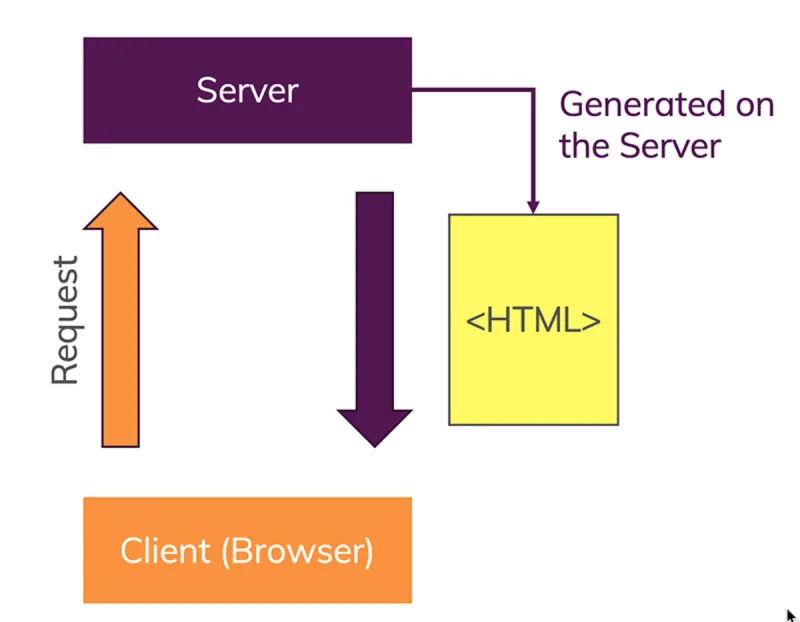
\includegraphics[width=.5\textwidth]{dynamic}  
    \caption{Dynamické vykreslování}
    \label{dynamic}
 \end{figure}

\hypertarget{statickuxe9-webovuxe9-struxe1nky}{%
\subsubsection{Statické webové stránky}\label{statickuxe9-webovuxe9-struxe1nky}}

Druhý přístup je nejstarší a~zároveň nejjednodušší, protože se jedná o~již vytvořené HTML (spolu s~CSS a~JavaScriptem) soubory, které jsou neměnné. To znamená, že jsou tyto již připravené statické soubory uložené na serveru, kde očekávají request od klienta k~vykreslení. Jedná se tedy nejčastěji o~takové webové stránky, které jsou jednodušší a~neočekává se u~nich příliš mnoho interaktivity s~uživatelem.

V~dnešní době jsou navíc populární takzvané generátory statických stránek, které umožňují vytvářet statické stránky na základě předpřipravených šablon a~odlehčeného značkovacího jazyka jako je například Markdown\footnote{https://www.markdownguide.org/}, v~němž se vytváří samostatný obsah~\parencite{spa}.

\begin{figure}[ht]   
    \centering
    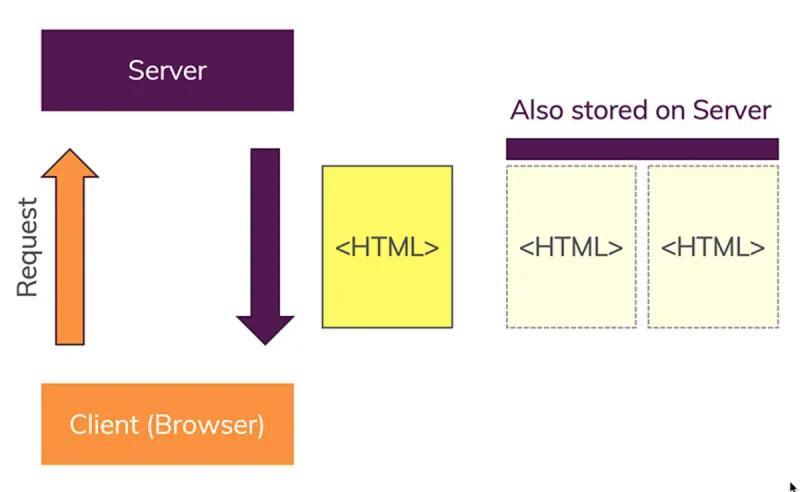
\includegraphics[width=.5\textwidth]{static}  
    \caption{Statické vykreslování}
    \label{static}
 \end{figure}

\hypertarget{single-page-applications}{%
\subsubsection{Single Page Applications}\label{single-page-applications}}

Posledním populárním přístupem jsou takzvané Single Page Applications (SPA), jejichž princip je přesně opačný od dynamických webových stránek. Klient sice také musí poslat request na server, nicméně ten vrací vždy jeden stejný HTML soubor s~velkým množství přidruženého javaScriptového kódu. JavaScript pak v~prohlížeči upravuje samotný DOM HTML souboru do výsledné podoby pro vykreslení.

Díky této strategii jsou webové stránky tohoto typu vysoce uživatelsky přívětivé, protože se veškeré vizuální změny dějí na klientovi. Pokud je tedy zapotřebí například stáhnout data z~databáze, JavaScript změní DOM do určité formy vizuálně přívětivého načítání nebo umožní data stahovat v~pozadí a~uživatel se může v~aplikace dál pohybovat. V~předchozích případech by návštěvník webu musel čekat, až se všechny změny provedou na serverové části.

Tento přístup má dvě základní nevýhody. Zaprvé může být v~některých případech pro prohlížeč náročné zpracovat všechny javaScriptové instrukce pro vygenerování výsledného HTML (zvláště, pokud jsou SPA neefetkivně napsané nebo uživatel používá starší zařízení / má pomalejší připojení). Druhým problémem bývá již zmíněné SEO -- iniciální HTML soubor totiž obsahuje malé množství metadat a~dalších informací o~stránce (jelikož ještě neproběhlo generování JavaScriptem) a~pro prohlížeč se webová stránka nemusí jevit důvěryhodně a~přiřazuje ji tak menší váhu při vyhledávání~\parencite{spa}.

\begin{figure}[ht]   
    \centering
    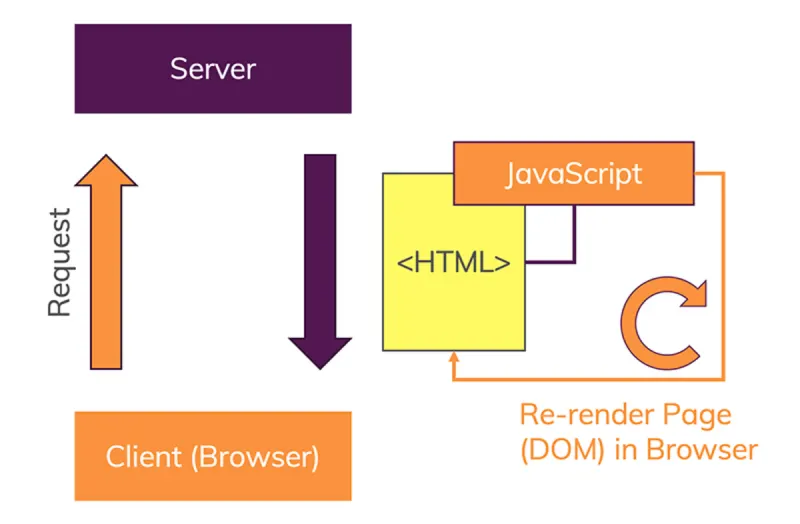
\includegraphics[width=.5\textwidth]{spa}  
    \caption{Single Page Application}
    \label{spa}
 \end{figure}

Jelikož naše aplikace obsahuje komplexnější komponenty, které nebývají součástí základních webových stránek (např. mapa pro geografické zobrazování), a~počítá s~vyšší mírou uživatelské interakce (např. administrační prostředí spolu s~autentifikací), volíme právě tento přístup pro vývoj našeho řešení.

\hypertarget{react}{%
\subsection{React}\label{react}}

Jak bylo výše napsáno, vývoj SPA aplikací je především záležitostí programování javaScriptového kódu. Aby nemuseli vývojáři veškerou integraci a~tvorbu základních funkcionalit tvořit stále od začátku, existují takzvané webové frameworky. Jejich hlavní význam je zjednodušit a~zefektivnit vývoj uživatelského rozhraní (frameworky samozřejmě existují i~pro ostatní části vývoje, například pro backend atd.) a~nastavují tak daným komunitám vývojářů základní pravidla, a~tím pádem určitou konzistenci pro strukturalizaci kódu. Tento aspekt je zvláště důležitý, pokud na určitém projektu pracuje větší množství lidí.

V~našem případě byly jedním z~nejdůležitějších nefunkčních požadavků udržitelnost a~rozšiřitelnost. Proto za webový framework vybíráme React\footnote{I přes to, že v~našem textu React popisujeme jako webový framework, není tomu zcela tak. Zcela přesně se jedna o~webovou knihovnu, která má mírně odlišné charakteristiky (např. výkon, komplexita atd.), nicméně pro naše účely můžeme tyto významové nuance ignorovat.}, který je v~tuto chvíli stále nejpopulárnější volbou mezi vývojáři na celém světě\footnote{https://www.developer-tech.com/news/2021/aug/03/2021-stack-overflow-survey-react-js-takes-the-web-framework-crown-python-is-in-demand-and-devs-still-love-rust/} a~základní znalost tohoto nástroje je tak v~dnešní době pro webové vývojáře takřka podmínkou.

Jedná se o~open-source software\footnote{https://github.com/facebook/react} vytvořený v~roce 2013 a~udržovaný programátory společností Meta (dříve Facebooku) za podpory široké komunity vývojářů~\parencite{react}.

React je založen na deklarativním vývoji uživatelského rozhraní. Vývojář tedy vytváří vzhled pro všechny stavy aplikace, které se pak vykreslují na základě změny v~datech (např. u~přihlášeného uživatele není zapotřebí zobrazovat tlačítko přihlášení a~naopak). Kód je tak pochopitelnější a~jednodušší na ladění chyb (debugging).

Druhou významnou vlastností Reactu je přístup založený na komponentách. Jedná se o~opakovaně použitelné části UI (tzn. i~samotného naprogramovaného kódu), které jsou hierarchicky strukturované buď podle využití v~aplikaci (např. adresář s~komponentou pro přihlášení \emph{Login} bude obsahovat soubor podkomponenty pro tlačítko \emph{LoginButton}), nebo podle obecně sdílených funkcionalit (všechny komponenty tlačítek v~aplikaci budou ve vlastní složce \emph{Buttons}). Data, na kterých jsou závislé jednotlivé stavy, lze mezi komponentami předávat prostřednictvím objektu s~názvem \emph{props}.

React namísto klasického stromové objektu DOM (viz \ref{zuxe1kladnuxed-webovuxe9-technologie}) využívá koncept virtuálního DOM (virtual Document Object Model). Jedná se o~speciální objektovou strukturu uloženou v~mezipaměti prohlížeče, která umožňuje efektivněji synchronizovat změny v~UI s~daným stavem aplikace. Zjednodušeně řečeno jde o~odlehčenou verzi DOM, s~níž lze na úrovni klienta jednodušeji manipulovat a~přizpůsobovat akcím od uživatele.

Posledním důležitým specifikem tohoto webového frameworku je využívání jazyka JSX, který je doporučován pro zápis komponent. JSX je svojí syntaxí nadstavbou JavaScriptu a~kombinuje strukturní značky, které známe z~HTML s~javaScriptovými konstrukcemi pro práci s~proměnnými a~funkcemi/metodami.

\hypertarget{typescript}{%
\subsection{TypeScript}\label{typescript}}

V~předchozí podkapitolách jsme popisovali významnou roli JavaScriptu při vývoji webových aplikací, nicméně existuje modernější a~vhodnější varianta tohoto programovacího jazyka -- TypeScript. Nejedná se ale o~nový, samostatný jazyk, ale o~rozšíření syntaxe stávajícího JavaScriptu. TypeScript byl vytvořen v~roce 2012 společností Microsoft a~jeho hlavním cílem je obohatit JavaScript o~typovou kontrolu objektů a~proměnných. Pomocí typové kontroly lze docílit k~větší prevenci potenciálních chyb a~celý kód se tak navíc stává přehlednějším~\parencite{typescript}.

Jelikož se chceme držet zásad čitelného a~čistého kódu, použijeme TypeScript i~v~naší aplikaci. Zároveň je zapotřebí dodat, že je javaScriptová syntaxe podmnožinou TypeScriptu\footnote{Typescript se vždy před spuštěním nejprve převede do čistého JavaScriptu, proto lze v~TypeScriptu psát v~případě potřeby čistý javaScriptový kód.}, tedy pro TypeScript platí všechny informace, které se v~této práci vážou k~JavaScriptu.

\hypertarget{technologie-spojenuxe9-s-vizualizacuxed-komunit-na-mapux11b}{%
\subsection{Technologie spojené s~vizualizací komunit na mapě}\label{technologie-spojenuxe9-s-vizualizacuxed-komunit-na-mapux11b}}

Hlavní součástí aplikace je vizualizace jednotlivých českých komunit po celém světě. Mapovými podklady (spolu s~nástroji, které s~mapou manipulují) standardně webové frameworky nedisponují. Níže popisujeme technologie, které jsme vybrali a~integrovali do našeho řešení.

\hypertarget{openstreetmap}{%
\subsubsection{OpenStreetMap}\label{openstreetmap}}

Za mapové podklady jsme vybrali volně editovatelné a~otevřené topografické mapy OpenStreetMap. Jedná se o~projekt, který vznikl v~roce 2004 jako protiváha proti tehdejším proprietárním řešením. Byl inspirován úspěchem Wikipedie a~jeho cílem je distribuovat volně dostupná geografická data jak pro nekomerční, tak komerční účely~\parencite{open-street}. Z~těchto důvodu jsme OpenStreetMap vybrali i~do naší aplikace.

\hypertarget{leaflet}{%
\subsubsection{Leaflet}\label{leaflet}}

Pro manipulaci s~OpenStreetMap jsme využili open-source javaScriptovou knihovnu Leaflet\footnote{Autorem knihovny je Kyjevan Volodymyr Agafonkin, který kvůli ruské invazi v~roce 2022 stejně jako mnoho ostatních Ukrajinců utekl ze svého domova. Téma této práce se týká i~nucených emigrací, a~proto si zde dovolíme udělat menší vložku a~vepsat odkaz, kde je možné podpořit Ukrajinu v~této nelehké době – https://www.comebackalive.in.ua/.}. Tento nástroj umožňuje webovým vývojářům vizualizovat na mapových podkladech vlastní interaktivní značky, vrstvy a~další vizuální prvky bez znalosti GIS\footnote{https://education.nationalgeographic.org/resource/geographic-information-system-gis}~\parencite{leaflet}.

Integrace nástroje Leaflet do frameworku React jsme provedli prostřednictvím knihovny React Leaflet. Ta je nástavbou předchozí knihovny a~abstrahuje jednotlivé složky Leafletu do systému komponent a~stavů, které jsou typické pro React~\parencite{react-leaflet}.

\hypertarget{geojson}{%
\subsubsection{GeoJSON}\label{geojson}}

Abychom byli schopni vkládat do OpenStreetMap prostřednictvím Leafletu vlastní geografická data krajanských komunit, musíme zvolit vhodný formát dat. Přenos dat ve světě webových technologií standardně probíhá pomocí formátu JSON (JavaScript Object Notation). Jde o~otevřený standard pro výměnu dat, který používá čitelný zápis skládající se vždy z~dvojic klíč -- hodnota. I~přes to, že je použitelný napříč programovacími jazyky, vychází z~JavaScriptu, konkrétně ze zápisu objektů (což je výhodné, protože se dá z~dat ihned vytvořit objekt a~dále s~nimi pracovat jako s~proměnnou). Jeho použití je rozmanité, nicméně se s~ním lze nejčastěji setkat při komunikaci mezi webovými aplikacemi a~vzdálenými servery~\parencite{json}.

GeoJSON z~formátu JSON vychází -- jedná se tedy o~otevřený standard pro reprezentaci takzvaných \emph{features} (OpenGIS standard pro specifikaci geografických dat). Pod \emph{features} si můžeme představit konkrétní tvary na mapě jako jsou například body, čáry, ale hlavně mnohoúhelníky, které využíváme pro vizualizaci lokalit~\parencite{geojson}.

Detailní tvorba \emph{features} ve formátu GeoJSON může být v~textovém editoru komplexní a~časově náročnou aktivitou. Jelikož je našim cílem editovat lokality v~aplikaci uživatelsky přívětivým způsobem, využíváme externí službu Geoman.io, která disponuje již vytvořeným GeoJSON editorem~\parencite{geoman}.

\hypertarget{firebase}{%
\subsection{Firebase}\label{firebase}}

Z~funkčních požadavků dále vyplývá potřeba ukládat data na vzdálenou databázi, aby byly informace pro všechny uživatele konzistentní a~aktualizované. Pro naplnění tohoto nároku jsme se rozhodli vybrat platformu Firebase od firmy Google, která nabízí předpřipravená cloudová řešení pro backendovou část (správa databáze a~autentifikace atd.) u~mobilních a~webových aplikací~\parencite{firebase}. Pro naše potřeby jsme využili tři nástroje popsané níže.

\hypertarget{firebase-authentication}{%
\subsubsection{Firebase Authentication}\label{firebase-authentication}}

Firebase Authentication je služba, která poskytuje komplexní řešení autentifikace v~souladu se základními standardy, jako jsou OAuth 2.0 and OpenID. Výhodou tohoto řešení je její integrace i~do ostatních Firebase produktů, je tedy možné např. nastavovat práva pro konkrétní přihlášené/nepřihlášené uživatele týkající se zápisu do Cloud Firestore databáze.

Nástroj nabízí registraci a~přihlašování přes různé poskytovatele, jako jsou Facebook, Google anebo Twitter, my ale využíváme klasického přihlášení přes e-mail a~heslo. V~této verzi aplikace nemá uživatel možnost vlastní registrace, protože administrační část je otevřena pouze ověřeným editorům krajanských komunit~\parencite{auth}.

\hypertarget{cloud-firestore}{%
\subsubsection{Cloud Firestore}\label{cloud-firestore}}

Druhým využitým nástrojem je Cloud Firestore -- databázové řešení, v~němž ukládáme všechna data textové povahy. Jedná se o~flexibilní a~škálovatelnou dokumentovou databázi, která ukládá data do kolekcí a~izolovaných JSON dokumentů (tzn. uložená data jsou až na pár detailů velmi podobná formátu, který využíváme v~naší aplikaci). Tuto databázi využíváme jako hlavní uložiště pro jednotlivé lokality~\parencite{firestore}.

\hypertarget{cloud-storage}{%
\subsubsection{Cloud Storage}\label{cloud-storage}}

Poslední zvolenou službou je Cloud Storage. Jde o~jednoduché a~cenově výhodné cloudové uložiště, které je uzpůsobeno k~ukládání netextových souborů jako jsou obrázky, audio soubory či videa. Tento nástroj umožňuje efektivní stahování a~nahrávání větších souborů spolu s~jejich validací a~kontrolou existence. Taktéž je navázán na Firebase Authentication, a~lze tak regulovat přístup k~některým souborům. Výhodou tohoto řešení je vysoká míra škálovatelnosti, kterou je zapotřebí řešit při větším počtu aktivních uživatelů~\parencite{storage}.

\hypertarget{data-o-krajanskuxfdch-komunituxe1ch}{%
\section{Data o~krajanských komunitách}\label{data-o-krajanskuxfdch-komunituxe1ch}}

Jelikož jsou data nutnou součástí a~vlastně i~samotným smyslem aplikace, popisujeme v~následující podkapitole strukturu a~obsah dat, ze kterých se skládají informace o~jednotlivých krajanských komunitách.

Zároveň platí, že všechny zmíněné složky lze v~administrativní části upravovat. Kromě názvu hlavní lokality a~geografických dat není žádná z~položek povinná, protože u~každé komunity nemusí být dostupné všechny typy informací. Pro větší přehlednost tyto informace dělíme do podsekcí tak, jak je lze najít v~administraci webové aplikace.

\hypertarget{uxfavod}{%
\subsection{Úvod}\label{uxfavod}}

\begin{itemize}
\tightlist
\item
  \textbf{Název hlavní lokality} -- jedná se o~unikátní název, bez kterého nelze lokalitu vytvořit. Podle hlavního názvu je komunita tříděna v~seznamu lokalit;
\item
  \textbf{Název sekundární lokality } -- doplňující název pro vyšší správní jednotky, tedy pro region, kraj nebo stát;
\item
  \textbf{Úvodní obrázek} -- náhledový obrázek, kterým je lokalita znázorněna ve vedlejším seznamu anebo při rozkliku mapové vrstvy;
\item
  \textbf{Demografické údaje} -- základní údaje týkající se především demografie komunity. Taktéž jsou zde pro větší přehlednost vypsány hodnoty, podle kterých mohou být aplikovány filtry (viz \ref{geografickuxe1-data}).
\end{itemize}

\hypertarget{detailnuxed-informace}{%
\subsection{Detailní informace}\label{detailnuxed-informace}}

\begin{itemize}
\tightlist
\item
  \textbf{Nahrávka}

  \begin{itemize}
  \tightlist
  \item
    Audio nahrávka -- audio soubor s~nahrávkou, která obsahuje příklad autentického jazyka vybrané české komunity;
  \item
    Název nahrávky a~případný komentář ke vzniku -- název audio nahrávky s~případným doprovodný komentářem;
  \item
    Přepis nahrávky -- fonetická transkripce zvukové nahrávky do textové podoby (bez použití speciálních znaků);
  \item
    Poznámky k~jazyku a~jazyková charakteristika -- komentář k~jazyku nahrávky a~popis jazykové charakteristiky komunity (hláskosloví, tvarosloví atd.);
  \item
    Další zdroje -- prostor pro odkazy na jazykovou normu či jiné zdroje.
  \end{itemize}
\item
  \textbf{Historie a~současnost}

  \begin{itemize}
  \tightlist
  \item
    Historie -- sekce určená k~popisu historie komunit;
  \item
    Současnost -- text věnovaný k~aktuálnímu stavu české enklávy.
  \end{itemize}
\end{itemize}

\hypertarget{multimediuxe1lnuxed-obsah}{%
\subsection{Multimediální obsah}\label{multimediuxe1lnuxed-obsah}}

\begin{itemize}
\tightlist
\item
  \textbf{Autor fotografií/obrázků} -- jméno a~případně odkaz na autora obrázků a~fotografií;
\item
  \textbf{Obrázky} -- libovolné množství fotografií a~dalších ilustračních obrázků dané české komunity spolu s~krátkými popisky;
\item
  \textbf{Audio} -- libovolné množství audio nahrávek s~rozhovory s~krajany či odborníky na danou lokalitu (spolu s~krátkými popisky);
\item
  \textbf{Videa} -- libovolné množství odkazů na videa o~komunitě spolu s~popisky;
\item
  \textbf{Texty} -- prostor na ukázky textových materiálů, jako jsou úryvky z~knih, místních časopisů atd.;
\item
  \textbf{Ostatní} -- sekce na doplňující informace, které se nehodily umístit nikam jinam.
\end{itemize}

\hypertarget{ostatnuxed}{%
\subsection{Ostatní}\label{ostatnuxed}}

\begin{itemize}
\tightlist
\item
  \textbf{Projekty} -- informace o~existujících projektech, jež souvisejí s~vybranou lokalitou;
\item
  \textbf{Nabídky} -- vyjmenování případných nabídek spolupráce či jiných participací s~komunitou;
\item
  \textbf{Atrakce} -- doplňující informace týkající se lokálních atrakcí, přírodních památek nebo turistického vyžití na daném místě;
\item
  \textbf{Zajímavosti} -- dodatečné zajímavosti ohledně historie, demografie či tamější architektury atd.;
\item
  \textbf{Zdroje} -- prostor na vkládání všech zdrojů, jež byly využity pro tvorbu digitálního záznamu o~krajanské komunitě;
\item
  \textbf{Kontakt} -- kontakt na tvůrce konkrétního záznamu.
\end{itemize}

\hypertarget{geografickuxe1-data}{%
\subsection{Geografická data}\label{geografickuxe1-data}}

\begin{itemize}
\tightlist
\item
  \textbf{GeoJSON} -- pole pro vkládání jedné mapové vrstvy ve formátu GeoJSON. Na tomto místě je také příložen odkaz na službu Geoman.io, prostřednictvím které lze jednoduše kreslit jednotlivé mapové objekty a~generovat tak GeoJSON soubor;
\item
  \textbf{Podmínky pro třídění na mapě} -- všechny níže uvedené podmínky jsou ve formě polí výběru (\emph{selection box}), u~nichž lze vybírat libovolné množství hodnot (níže je vždy vedle názvu filtru vypisujeme). Podle těchto vybraných hodnot je pak možné lokality filtrovat na mapě a~v~bočním seznamu;

  \begin{itemize}
  \tightlist
  \item
    Doba příchodu česky mluvících osob

    \begin{itemize}
    \tightlist
    \item
      1550--1620,
    \item
      1620--1700,
    \item
      1700--1800,
    \item
      1800--1850,
    \item
      1850--1914,
    \item
      1914--1930,
    \item
      po 1939,
    \item
      po 1989;
    \end{itemize}
  \item
    Doba zániku

    \begin{itemize}
    \tightlist
    \item
      před 1620,
    \item
      před 1700,
    \item
      v~18. století,
    \item
      v~19. století,
    \item
      v~1. pol. 20. stol,
    \item
      ve 2. pol. 20. stol,
    \item
      2000--současnost;
    \end{itemize}
  \item
    Velikost komunity

    \begin{itemize}
    \tightlist
    \item
      méně než 10,
    \item
      10--50,
    \item
      více než 50,
    \item
      více než 500,
    \item
      více než 10 000,
    \item
      více než 50 000;
    \end{itemize}
  \item
    Převládající nářeční základ

    \begin{itemize}
    \tightlist
    \item
      městská mluva,
    \item
      severovýchodočeská skupina,
    \item
      středočeská,
    \item
      jihozápadněčeská skupina,
    \item
      středomoravská,
    \item
      východomoravská,
    \item
      lašská,
    \item
      českomoravská;
    \end{itemize}
  \item
    Počet generací, po které se čeština uchovala

    \begin{itemize}
    \tightlist
    \item
      1,
    \item
      2,
    \item
      3,
    \item
      4,
    \item
      5,
    \item
      6,
    \item
      7,
    \item
      8,
    \item
      9,
    \item
      10;
    \end{itemize}
  \item
    Převládající motivace pro emigraci z~českých zemí

    \begin{itemize}
    \tightlist
    \item
      náboženská (cca do 1850),
    \item
      hospodářská (1820--1939, po 1989),
    \item
      politická (zejm. po 1939--1989);
    \end{itemize}
  \item
    Existuje audiomateriál nebo písemná dokumentace jazyka?

    \begin{itemize}
    \tightlist
    \item
      ano,
    \item
      ne;
    \end{itemize}
  \item
    Převládající náboženství

    \begin{itemize}
    \tightlist
    \item
      protestantské,
    \item
      katolické,
    \item
      bez vyznání,
    \item
      nezjištěno;
    \end{itemize}
  \item
    Proběhla reemigrace?

    \begin{itemize}
    \tightlist
    \item
      po 1. světové válce,
    \item
      po 2. světové válce;
    \end{itemize}
  \item
    Typ migrace

    \begin{itemize}
    \tightlist
    \item
      primární,
    \item
      sekundární,
    \item
      další migrace.
    \end{itemize}
  \end{itemize}
\end{itemize}

\hypertarget{uux17eivatelskuxe9-rozhranuxed}{%
\section{Uživatelské rozhraní}\label{uux17eivatelskuxe9-rozhranuxed}}

V~následující podkapitole si na konkrétních ukázkách z~aplikace představíme průchod uživatelským rozhraním se zřetelem na nejdůležitější interakční prvky. Návrh celého rozhraní vychází z~funkčních požadavků.

Zároveň je zapotřebí dodat, že jsou v~době psaní této práce v~aplikaci přítomny dva kompletní záznamy krajanských komunit (Šumice a~Kirillovka), na nichž budeme demonstrovat funkčnost aplikace.

Na každé stránce aplikace je v~horní části umístěné statické navigační menu, přes které se uživatel může dostat do jednotlivých částí. Respektive pokud uživatel není přihlášen, vyskytuje se na konci panelu tlačítko pro přihlášení, v~případě že přihlášen je, se může pomocí návodné ikony odhlásit.

Vstupní částí aplikace je stránka s~mapou (viz obrázek \ref{mapa}), na níž jsou při defaultní pozici mapy vidět bodově označené lokality. V~mapové části se uživatel může pohybovat standardním způsobem a~pro navrácení pozice mapy do výchozího stavu lze využít tlačítko pod tlačítkem oddálení. Taktéž je v~pravém horním rohu umístěna miniaturní verze mapy pro přehlednější orientaci.

Práci s~mapou navíc usnadňuje vyhledávač, který má dvě hlavní funkce. Uživatel po jeho nakliknutí ihned uvidí všechny dostupné lokality českých komunit, nemusí je tak složitě zjišťovat ze seznamu a~vepisovat jejich jména (po výběru je pohled mapy ihned přesunut na vybranou lokalitu). Vyhledávač také umožňuje měnit výsek mapy na jakékoliv lokace, města a~regiony, které jsou v~běžných mapách dostupné (tato funkce navíc funguje napříč jazyky -- např. pohled mapy se přesune nad Paříž, pokud napíšeme do vyhledávače Paris, tak i~českou variantu Paříž).

\begin{figure}
    \centering
    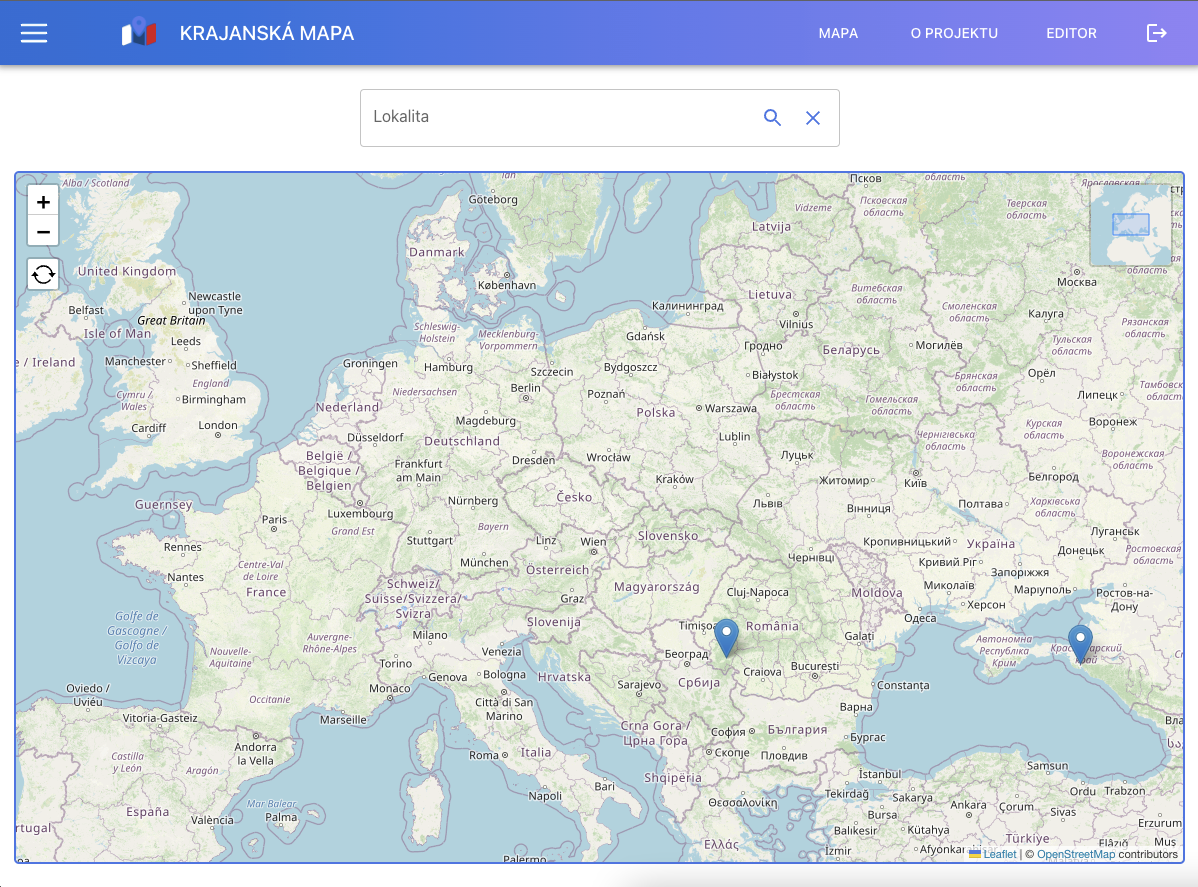
\includegraphics[width=0.95\textwidth]{mapa}  
    \caption{Výchozí pohled na mapu}
    \label{mapa}
\end{figure}

Výčet dostupných lokalit se zobrazuje prostřednictvím tlačítka menu v~levé části navigačního panelu. Tímto způsobem se zobrazí vysouvací postranní sekce s~abecedně seřazenými lokalitami podle aplikovaných filtrů (ve výchozím stavu bez omezení) (viz obrázek \ref{mapa-2}).

\begin{figure}  
    \centering
    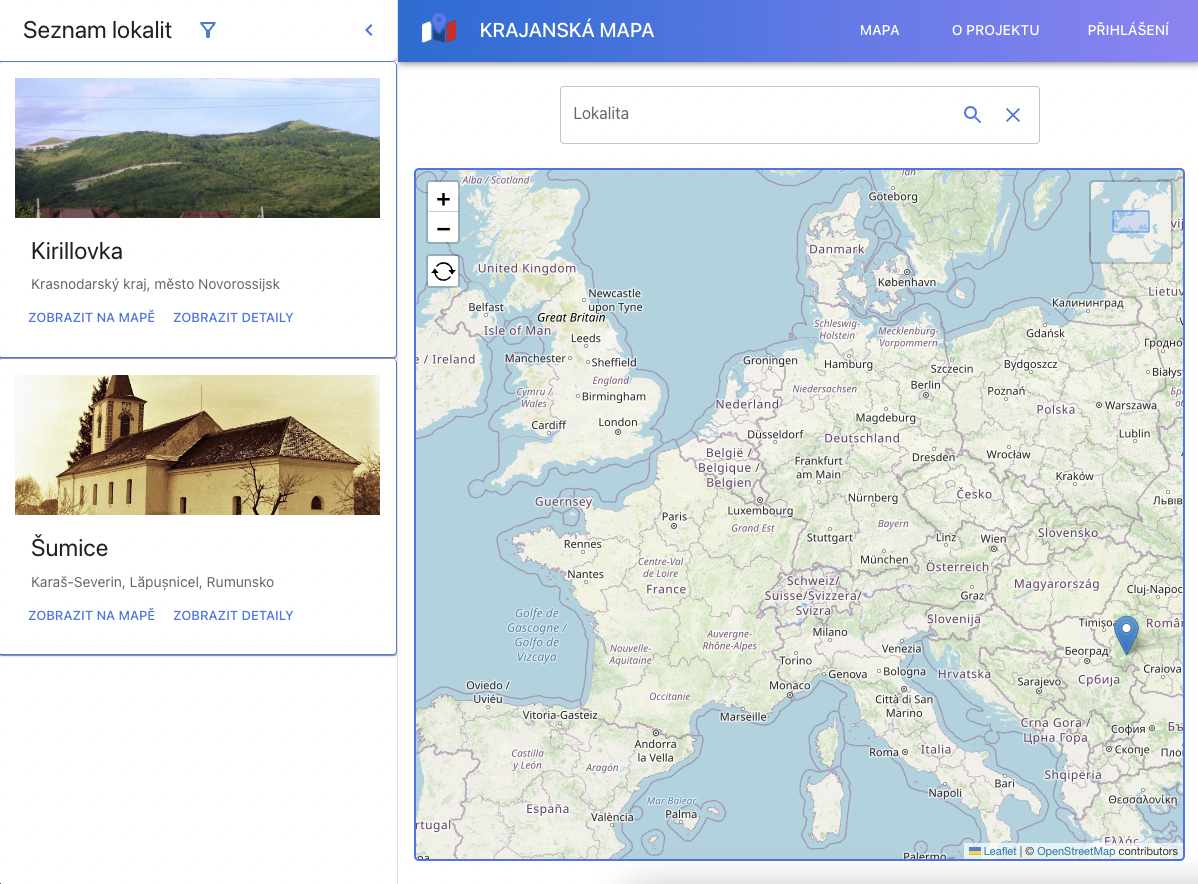
\includegraphics[width=0.95\textwidth]{mapa-2}  
    \caption{Seznam lokalit v~bočním panelu}
    \label{mapa-2}
\end{figure}

Nastavování filtrů se otevírá přes ikonu filtru vedle \emph{Seznamu lokalit}. Změní se tak mód vysouvacího panelu, kde můžeme zatrhávat libovolné množství podmínek pro zobrazení lokalit (viz obrázek \ref{filtr1}).

\begin{figure}
    \centering
    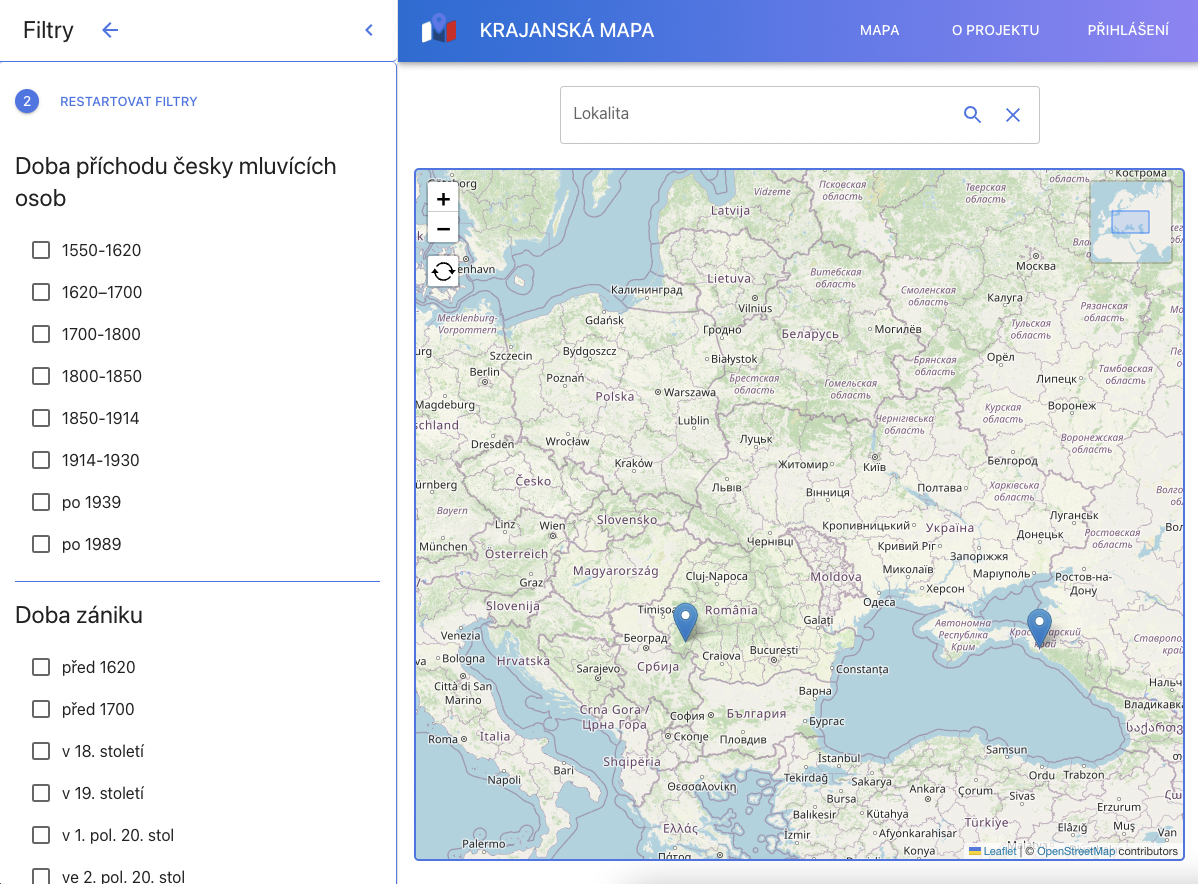
\includegraphics[width=0.95\textwidth]{filtr1} 
    \caption{Výchozí stav filtrů}
    \label{filtr1}
\end{figure}

Po výběru daných filtrů si uživatel může povšimnout okamžitě projevené změny zobrazení (viz obrázek \ref{filtr2}), a~to jak na mapě, tak i~v~předchozím seznamu lokalit (pro větší přehlednost je počet aktuálně vyfiltrovaných komunit zobrazen vedle možnosti \emph{Restartovat filtry}, uživatel má tak možnost ihned vidět celkový počet).

\begin{figure}  
    \centering
    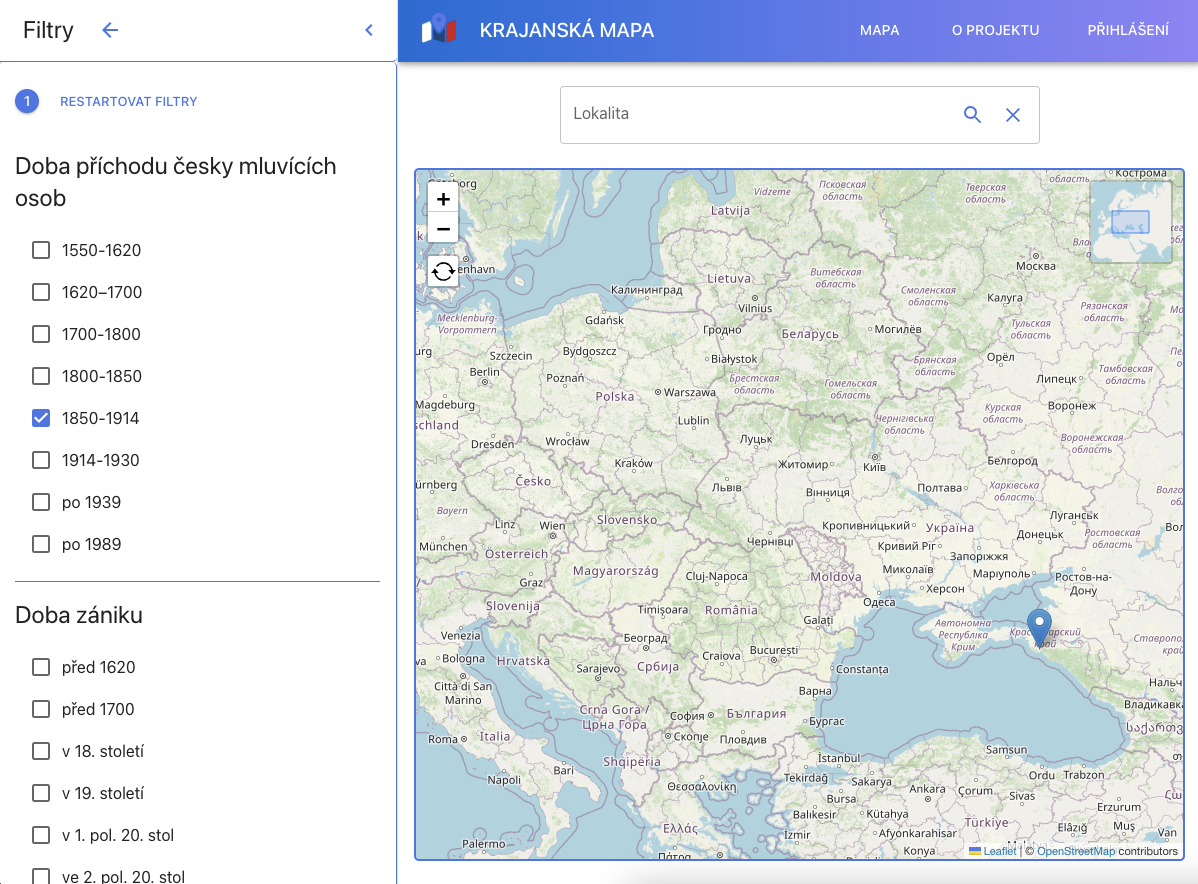
\includegraphics[width=0.95\textwidth]{filtr2}  
    \caption{Stav po použití filtru}
    \label{filtr2}
\end{figure}

Pro přiblížení na konkrétní krajanskou komunitu na mapě lze využít buď tlačítko \emph{Zobrazit na mapě} u~vybrané lokality (pokud je uživatel přihlášen, ja na tomto místě navíc umístěna ikona nastavení pro přechod na stránku s~administrací), případně kliknout na modrou značku, která je zobrazená na mapě. Po jednoduché animaci je pohled mapy zacílen na danou mapovou vrstvu (viz obrázek \ref{cil-mapa}).

Pokud by se vedle sebe nacházelo větší množství lokalit, lze je od sebe navzájem rozlišit po najetí myši na mapovou vrstvu -- vypíše se tak hlavní název komunity. Po kliknutí na mapovou vrstvu se zobrazí modální okno s~hlavním a~vedlejším názvem, případně s~úvodním obrázkem a~s~dalšími akcemi, jako jsou \emph{Upravit lokalitu} (v~případě přihlášení), \emph{Zpátky} a~\emph{Přejít na lokalitu}.

\begin{figure} 
    \centering
    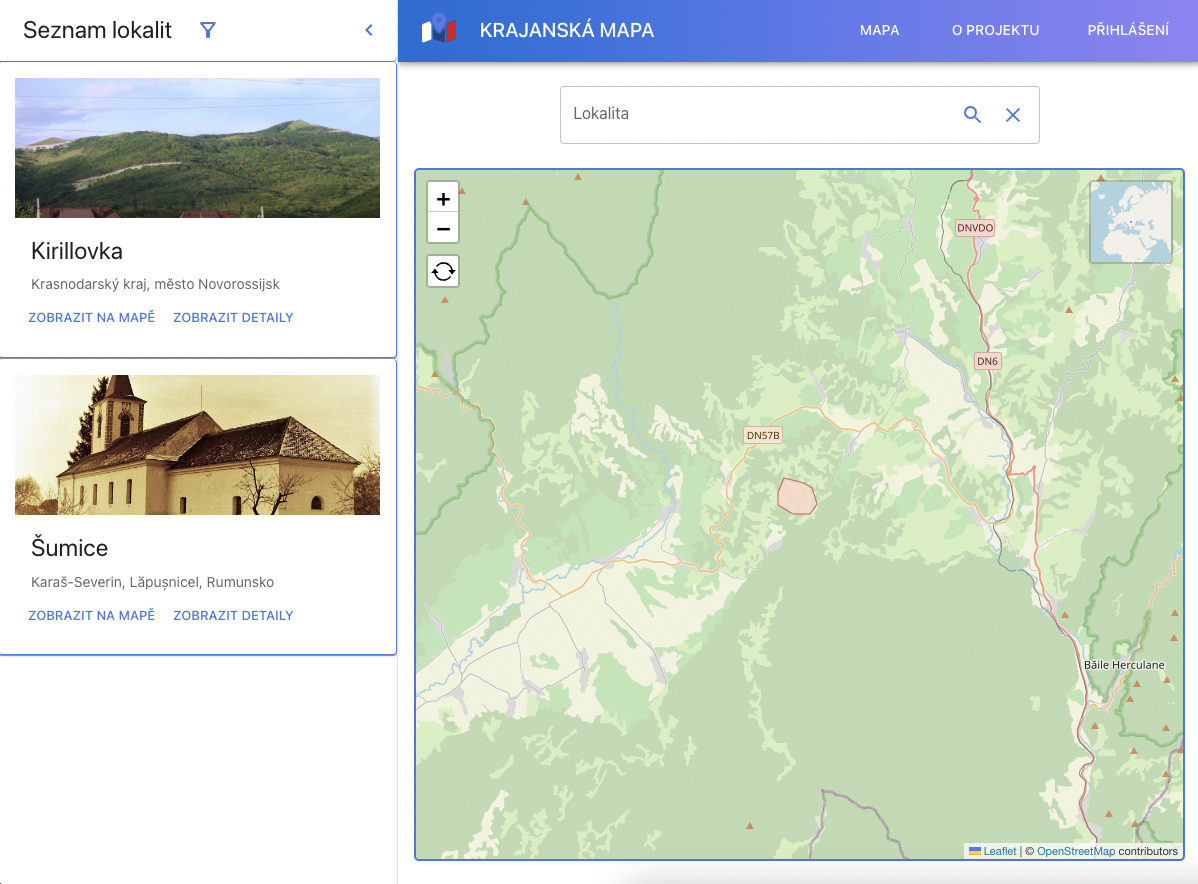
\includegraphics[width=0.95\textwidth]{cil-mapa}  
    \caption{Přiblížení na vybranou krajanskou komunitu}
    \label{cil-mapa}
\end{figure}

Jak bylo v~minulé podkapitole zmíněno, informace o~vybrané lokalitě se dělí do několika oddílů. První z~nich je úvodní stránka (viz obrázek \ref{uvod-obr}) se základními informaci.

V~druhé sekci můžeme najít audio nahrávku a~další informace, jež s~ní souvisí (viz obrázek \ref{detail}). V~okamžiku, kdy uživatel spustí audio přehrávač, zobrazí se i~případné jazykové informace, které se k~nahrávce vážou (transkripce, jazyková charakteristika atd.), ty lze ovšem dle potřeby skrýt. Pod nahrávkou jsou pak informace vztahující se k~jak historii, tak k~současné situaci dané komunity.

\begin{figure} 
    \centering
    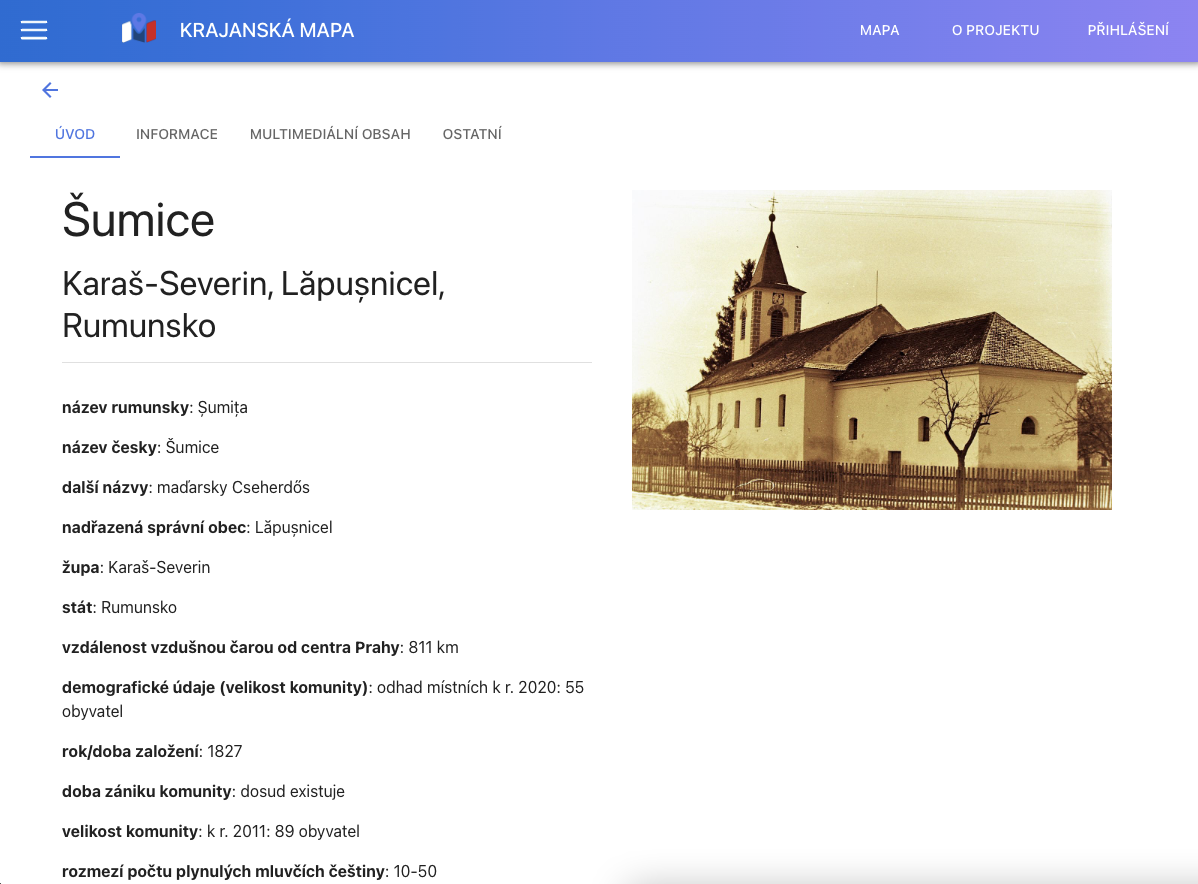
\includegraphics[width=0.95\textwidth]{uvod}  
    \caption{Úvodní informace}
    \label{uvod-obr}
\end{figure}

\begin{figure}
    \centering
    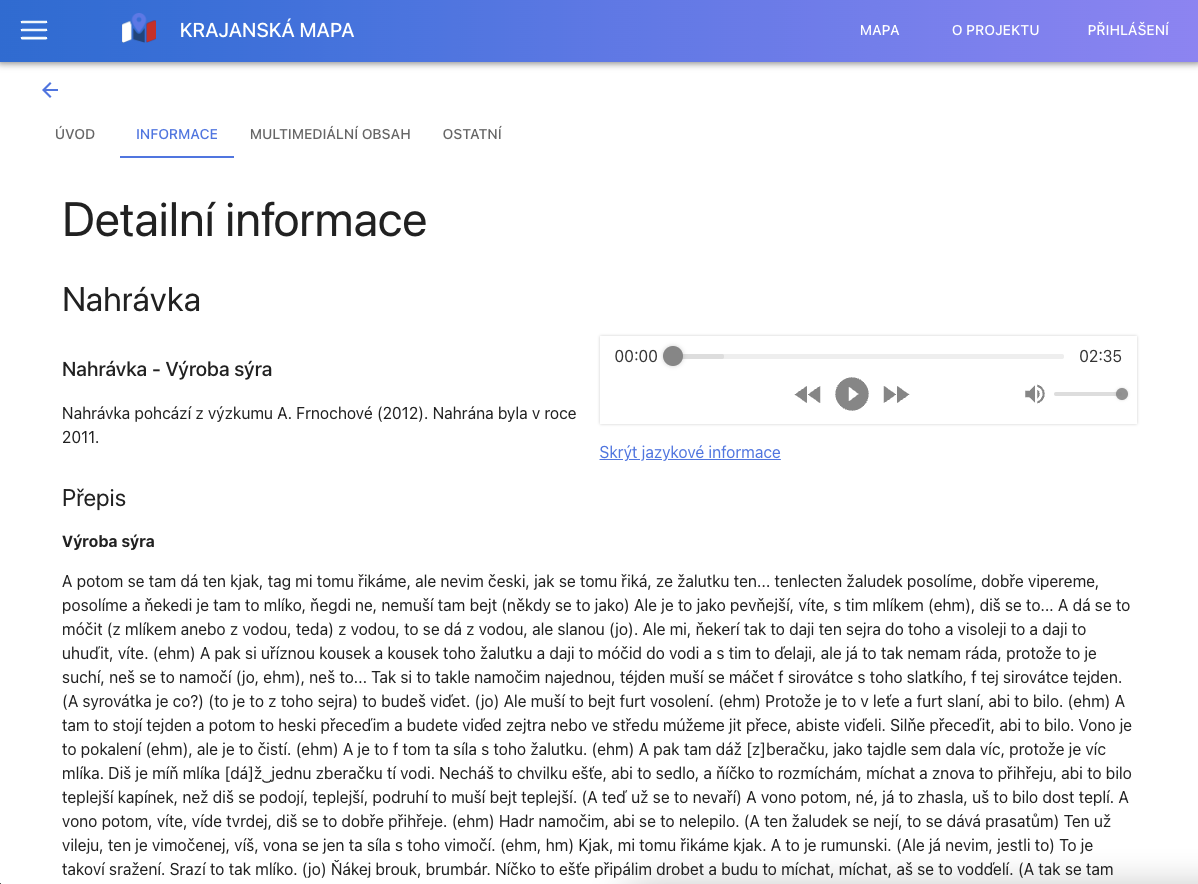
\includegraphics[width=0.95\textwidth]{detail}  
    \caption{Detailní informace spolu s~audio nahrávkou}
    \label{detail}
\end{figure}

Třetí část se skládá z~multimediálního obsahu. Pro zobrazení fotografií jsme vybrali uživatelsky přívětivou podobu obrázkové galerie, která v~sobě obsahuje náhled na všechny obrázkové soubory (viz obrázek \ref{media}). Také je zde možnost zobrazení na celou obrazovku nebo přepínání obrázků pomocí šípek na klávesnici. V~této sekci se taktéž případně nachází další audio nahrávky, přiložená videa ve formě vloženého YouTube přehrávače či libovolné množství textových materiálů.

Poslední oddílem je část \emph{Ostatní}, kde je prostor na jakékoliv dodatečné textové informace, jakou jsou projekty, nabídky, atrakce, zajímavosti (viz obrázek \ref{ostatni}). Zároveň je zde místo pro výpis použitých zdrojů a~název autora, který tento záznam vytvořil.

Užitečným detailem je v~tomto kontextu sdílení vybrané lokality prostřednictvím jejího URL odkazu na jiné zařízení\footnote{Například https://czech-map.netlify.app/location/Šumice.}. Aplikace podle názvu v~URL odkazu rozpozná danou komunitu a~stáhne si ze vzdálené databáze všechna potřebná data.

\begin{figure}  
    \centering
    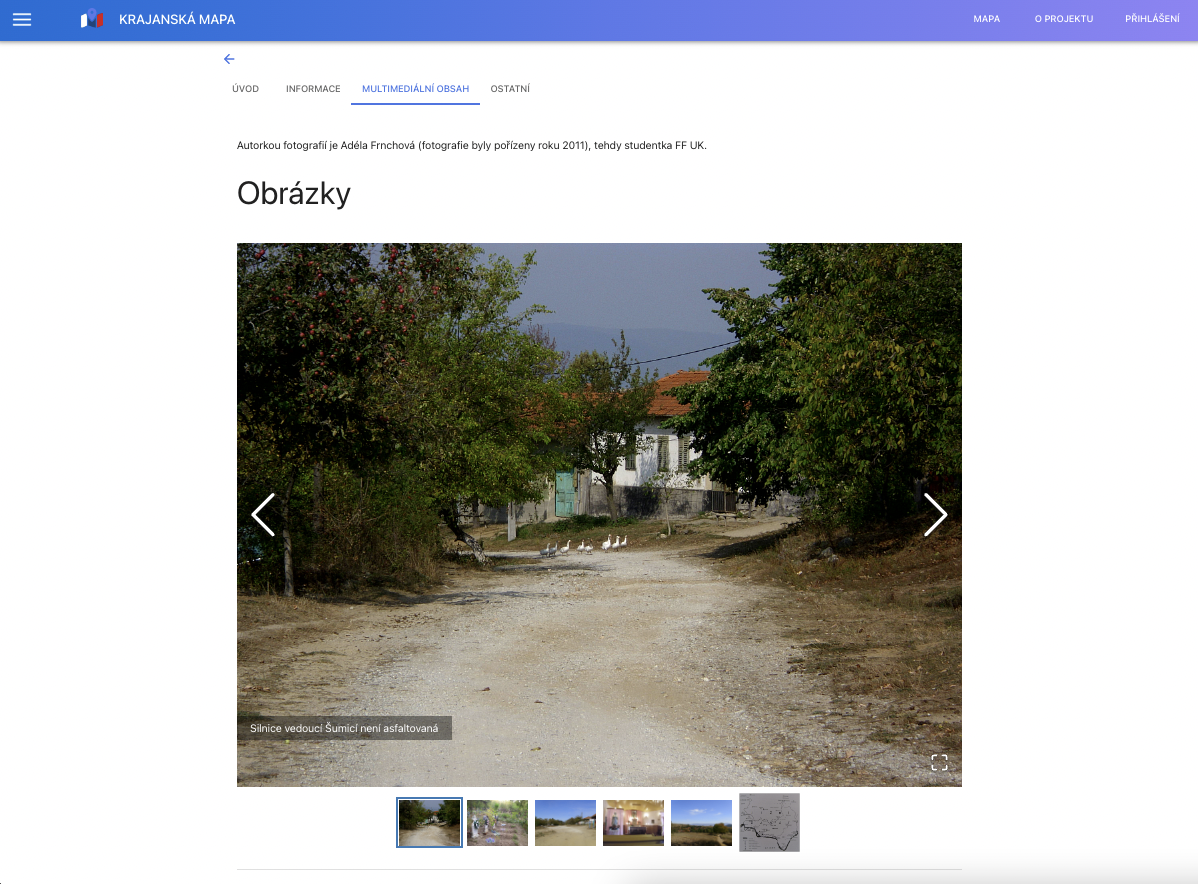
\includegraphics[width=0.95\textwidth]{media}  
    \caption{Obrázková galerie}
    \label{media}
\end{figure}

\begin{figure} 
    \centering
    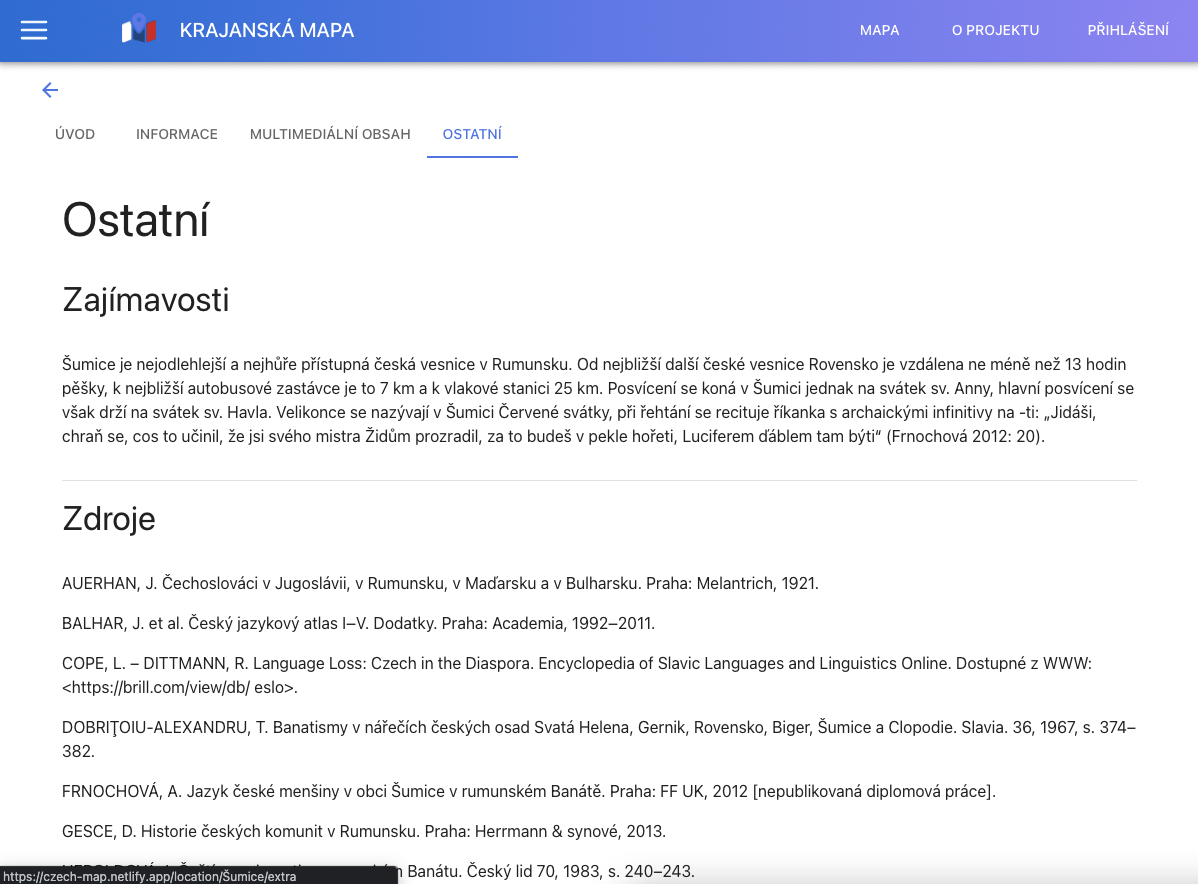
\includegraphics[width=0.95\textwidth]{ostatni}  
    \caption{Poslední část s~doplňujícími informacemi}
    \label{ostatni}
\end{figure}

Administraci lze otevřít až po úspěšném loginu na stránce \emph{Přihlášení} (viz obrázek \ref{login}) prostřednictvím přiřazeného e-mailu a~hesla. Uživatel v~tuto chvíli nemá možnost účet založit, pro editory krajanských komunit budou v~této fázi údaje zpřístupněny po případné domluvě.

\begin{figure}
    \centering
    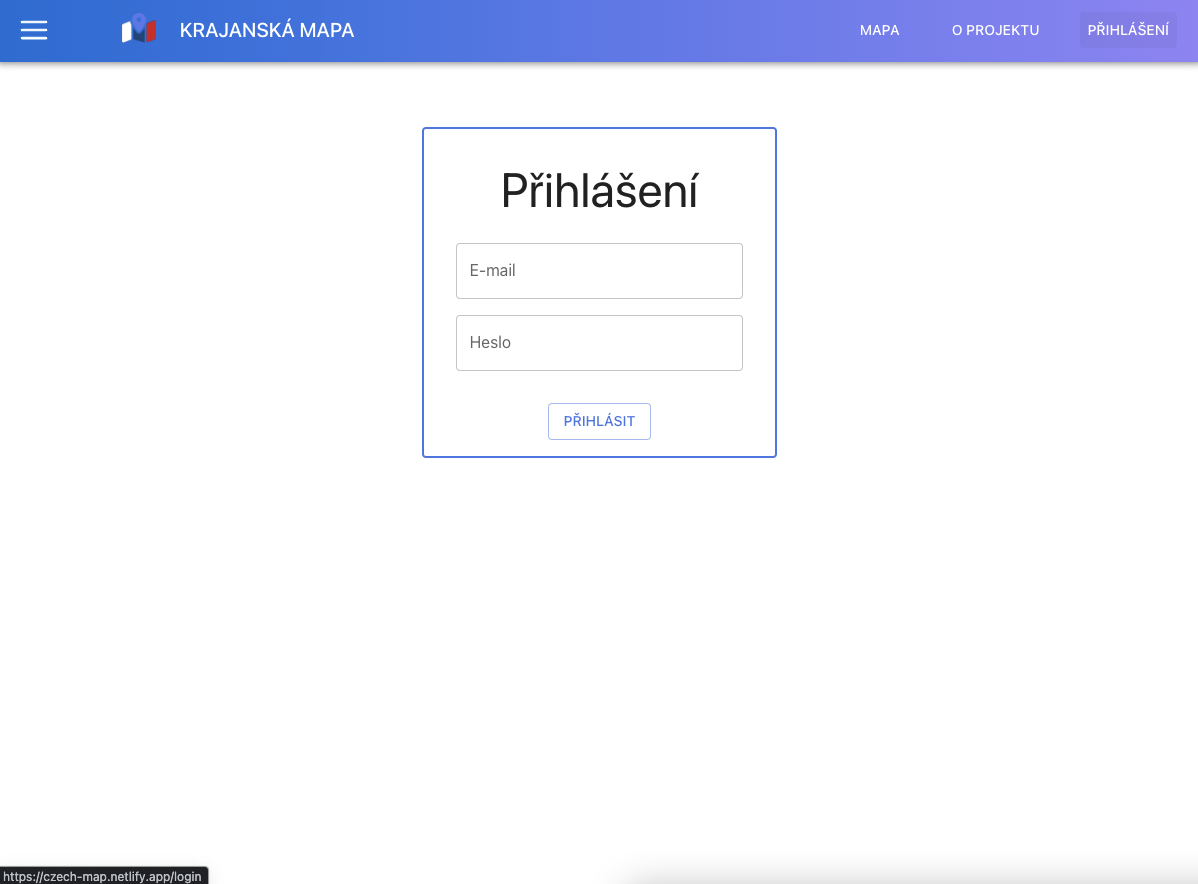
\includegraphics[width=0.95\textwidth]{login}  
    \caption{Přihlášení}
    \label{login}
\end{figure}

Po přihlášení se v~navigačním menu objeví nová položka \emph{Editor}, která uživatele přesměruje do podstránek s~administrací, kde probíhají všechny úkony spojené s~editací jednotlivých lokalit.

Stránku s~administrací lze použít dvěma základními způsoby. Buď vytvořit novou lokalitu (tedy kliknout na tlačítko v~menu), anebo použít některou z~možností pro úpravu již existujícího záznamu (např. v~seznamu lokalit, v~modálním okně či v~samotném detailu komunity). Níže představujeme administraci pro již existující komunitu.

Po přepnutí do administrace si uživatel může všimnout \emph{progress baru} (ukazatele průběhu) umístěného hned pod navigačním menu, který reaguje na přepnutí napříč sekcemi (tedy na začátku je téměř prázdný, v~posledním oddíle naopak plný) (viz obrázek \ref{admin-uvod}).

Pod tímto indikátorem jsou názvy oddílů, které je možné v~rámci editoru vyplňovat, a~následně dvě ikony pro vstup na lokalitu a~pro odstranění celého záznamu (před smazáním se objevuje konfirmační modální okno, kde musí uživatel svoji volbu potvrdit).

\begin{figure}
    \centering
    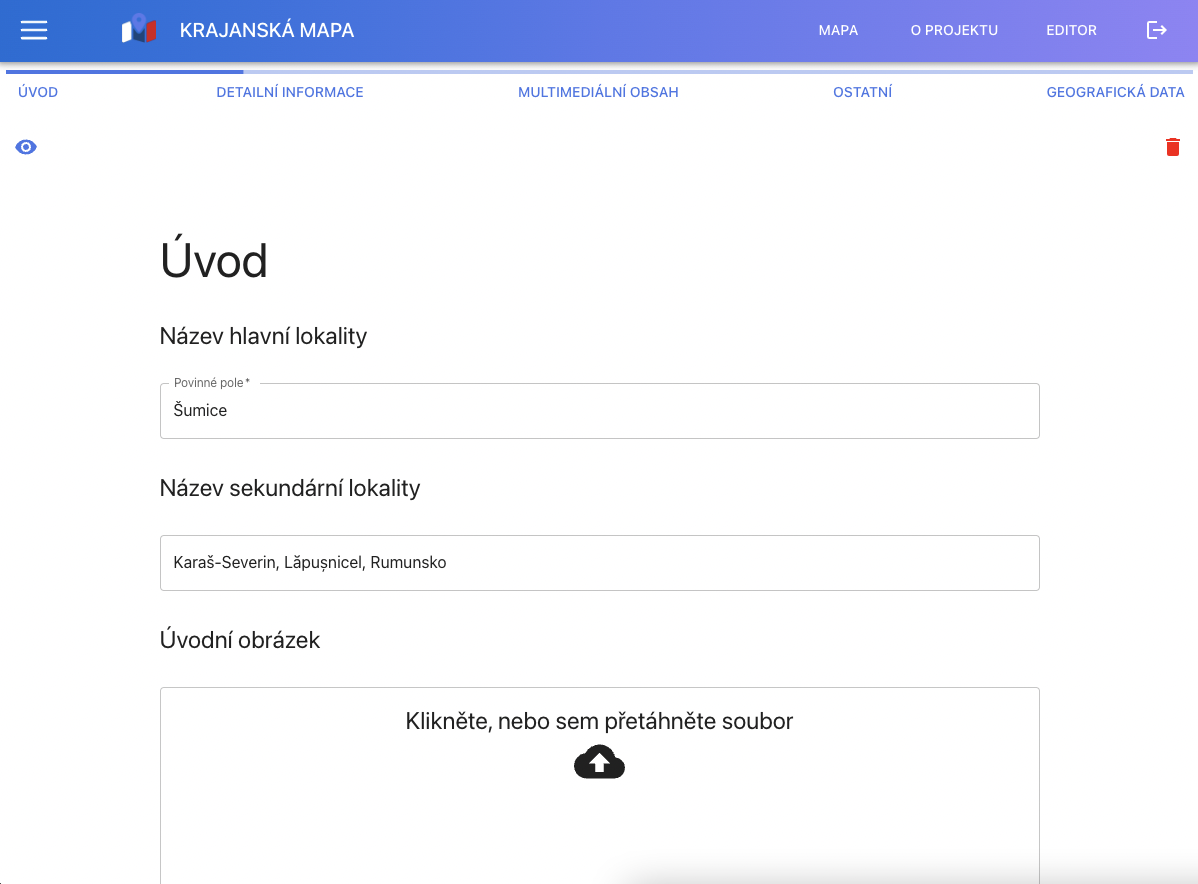
\includegraphics[width=0.95\textwidth]{admin-uvod}  
    \caption{Úvodní stránka administrace}
    \label{admin-uvod}
\end{figure}

Dále se pak nachází vždy obsah pro jednotlivé oddíly, kde je možné vyplňovat data pro vybrané položky. U~položek textového charakteru jsou prvky formuláře buď jednoduchého typu (umožňují vkládat text pouze bez formátování, například název atd.), anebo se jedná o~složitější textový editor pro uložení komplexnější textové informace (viz obrázek \ref{admin-nahravka}).

V~textovém editoru je možné přidávat standardní značky pro formátování textu, jako jsou odrážky, tučný řez písma, odkazy, nadpisy, ale i~třeba emotikony a~další prvky, které mohou být užitečné v~některých sekcích. Do aplikace tak lze jednoduše a~efektivně vkládat delší texty, které si uživatel připraví např. v~textovém procesoru typu MS Word.

\begin{figure}
    \centering
    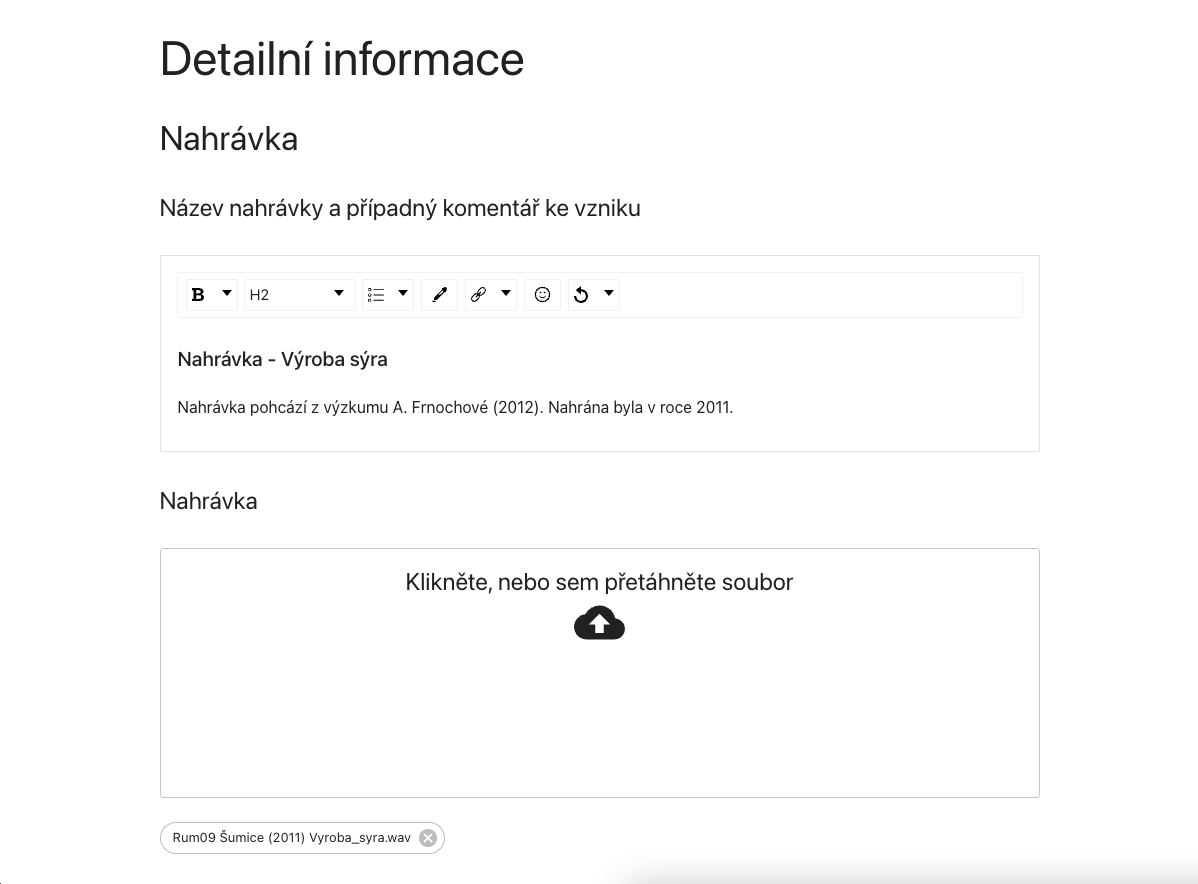
\includegraphics[width=0.95\textwidth]{admin-nahravka}  
    \caption{Prvky formuláře pro vkládání delšího textu a~audio nahrávky}
    \label{admin-nahravka}
\end{figure}

Pro vkládání souborů (obrázky a~audio) do systému pak slouží speciální komponenta, která přehledným způsobem vykresluje již vložené soubory ve formě textu (viz obrázek \ref{admin-obrazky}). Uživatel na první pohled vidí, jaké soubory jsou součástí dané lokality a~může tak jednoduchým způsobem přidávat a~odstraňovat soubory (či jejich popisky) dle potřeby.

\begin{figure}
    \centering
    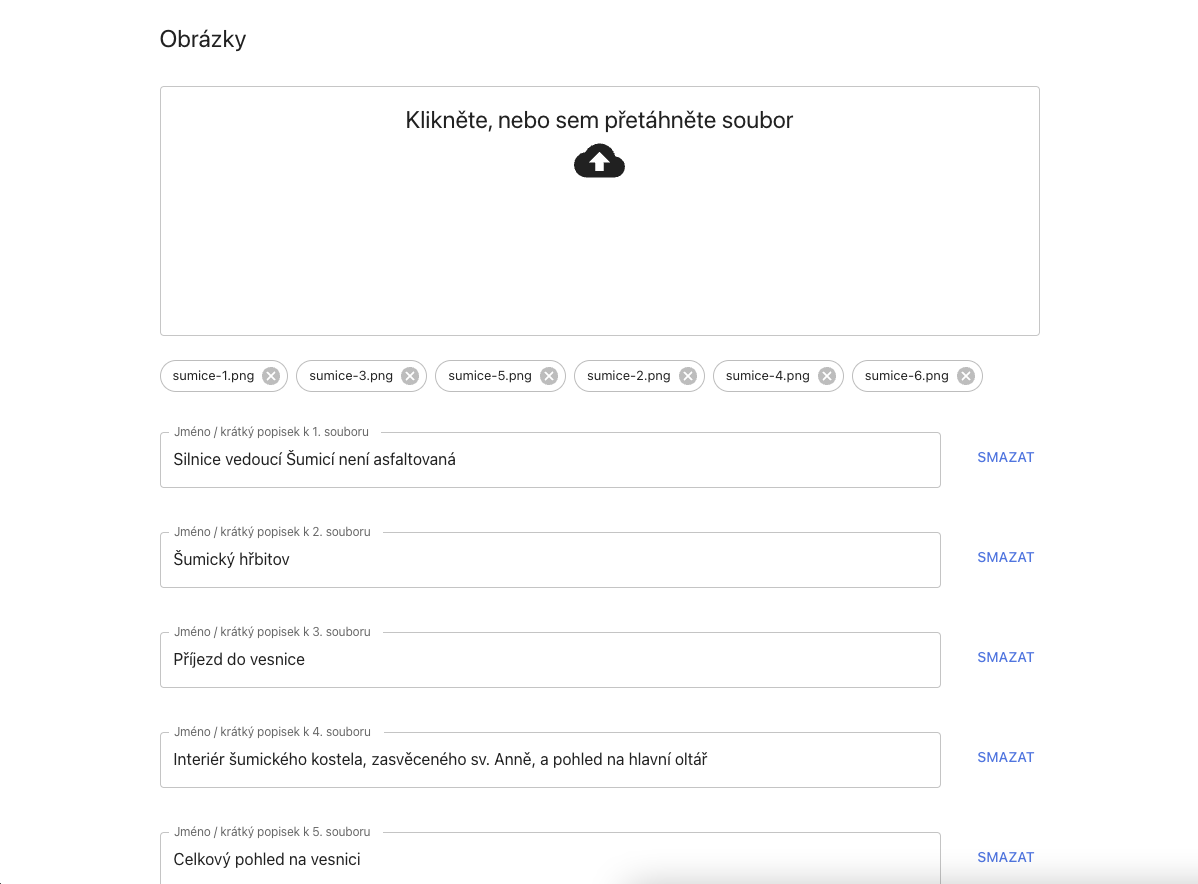
\includegraphics[width=0.95\textwidth]{admin-obrazky}  
    \caption{Vkládání obrázků přes speciální komponentu}
    \label{admin-obrazky}
\end{figure}

Poslední důležitou složkou administrace je správa geografických dat a~nastavování filtrů (viz obrázek \ref{admin-geo}). Jak bylo v~předchozí podkapitole zmíněno, geografická data aplikace zpracovává ve formátu GeoJSON. Proto využíváme speciálně upravený textový editor, který dokáže validovat správný formát vstupního textu (GeoJSON je i~přes svoje specifika v~principu stále textový řetězec).

Pravděpodobnost chyby se navíc snažíme eliminovat tím způsobem, že uživatele nutíme měnit obsah pole pouze prostřednictvím zkopírování textu. Takto chceme editora motivovat k~využití přiložené služby Geoman.io, kde si může jednoduchým způsobem nakreslit potřebnou mapovou vrstvu a~vygenerovat si tak GeoJSON kód (viz obrázek \ref{geoman}). Ten pak stačí celý zkopírovat a~rovnou vložit do naší aplikace, která jej pak automaticky zpracuje a~vybere z~něj potřebné hodnoty pro zakreslení do mapy.

Věříme, že tento způsob je v~této fázi aplikace uživatelsky nejpřívětivější a~efektivní zároveň. Jedinými nevýhodami tohoto přístupu jsou prozatímní závislost na externím nástroji a~nutnost při úpravě existující lokality znovu vygenerovat celý GeoJSON kód.

Volba filtrů je vytvořena jednoduchým způsobem skrze \emph{selection boxy} s~vícenásobným výběrem. V~závěru je zapotřebí data z~celé administrativní části odeslat pomocí výrazného tlačítka umístěného na konci stránky. Až pak se propíší do databáze a~zároveň do dalších částí aplikace. Je tedy zřejmé, že uživatel nesmí při editace ztratit připojení nebo jakýmkoliv jiným způsobem přerušit spojení s~editorem (např. aktualizace stránky atd.). I~z~tohoto důvodu je přidáno konfirmační modální okno po kliknutí na ikony oka, jež slouží pro zobrazení lokality ve standardním módu.

\begin{figure}
    \centering
    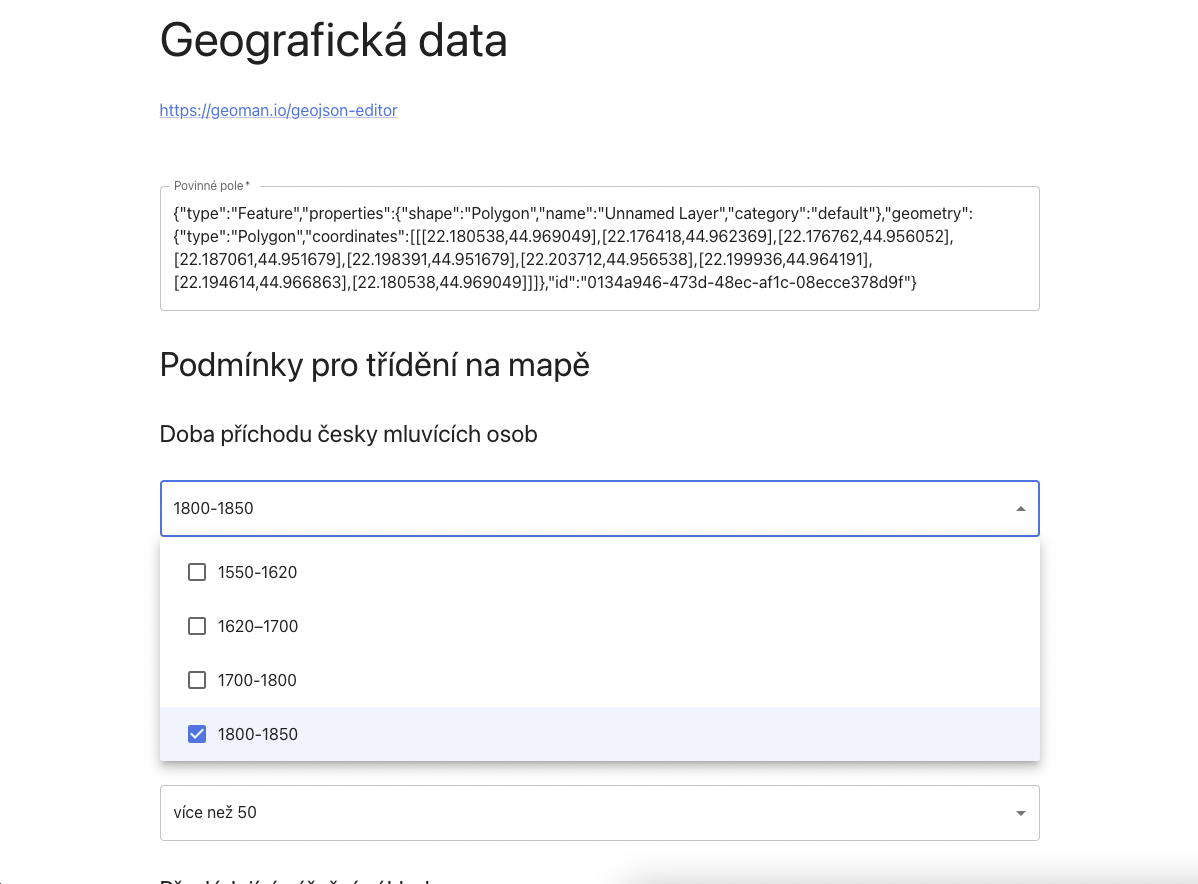
\includegraphics[width=0.95\textwidth]{admin-geo}  
    \caption{Vkládání geografických dat a~úprava filtrů}
    \label{admin-geo}
\end{figure}

\begin{figure}
    \centering
    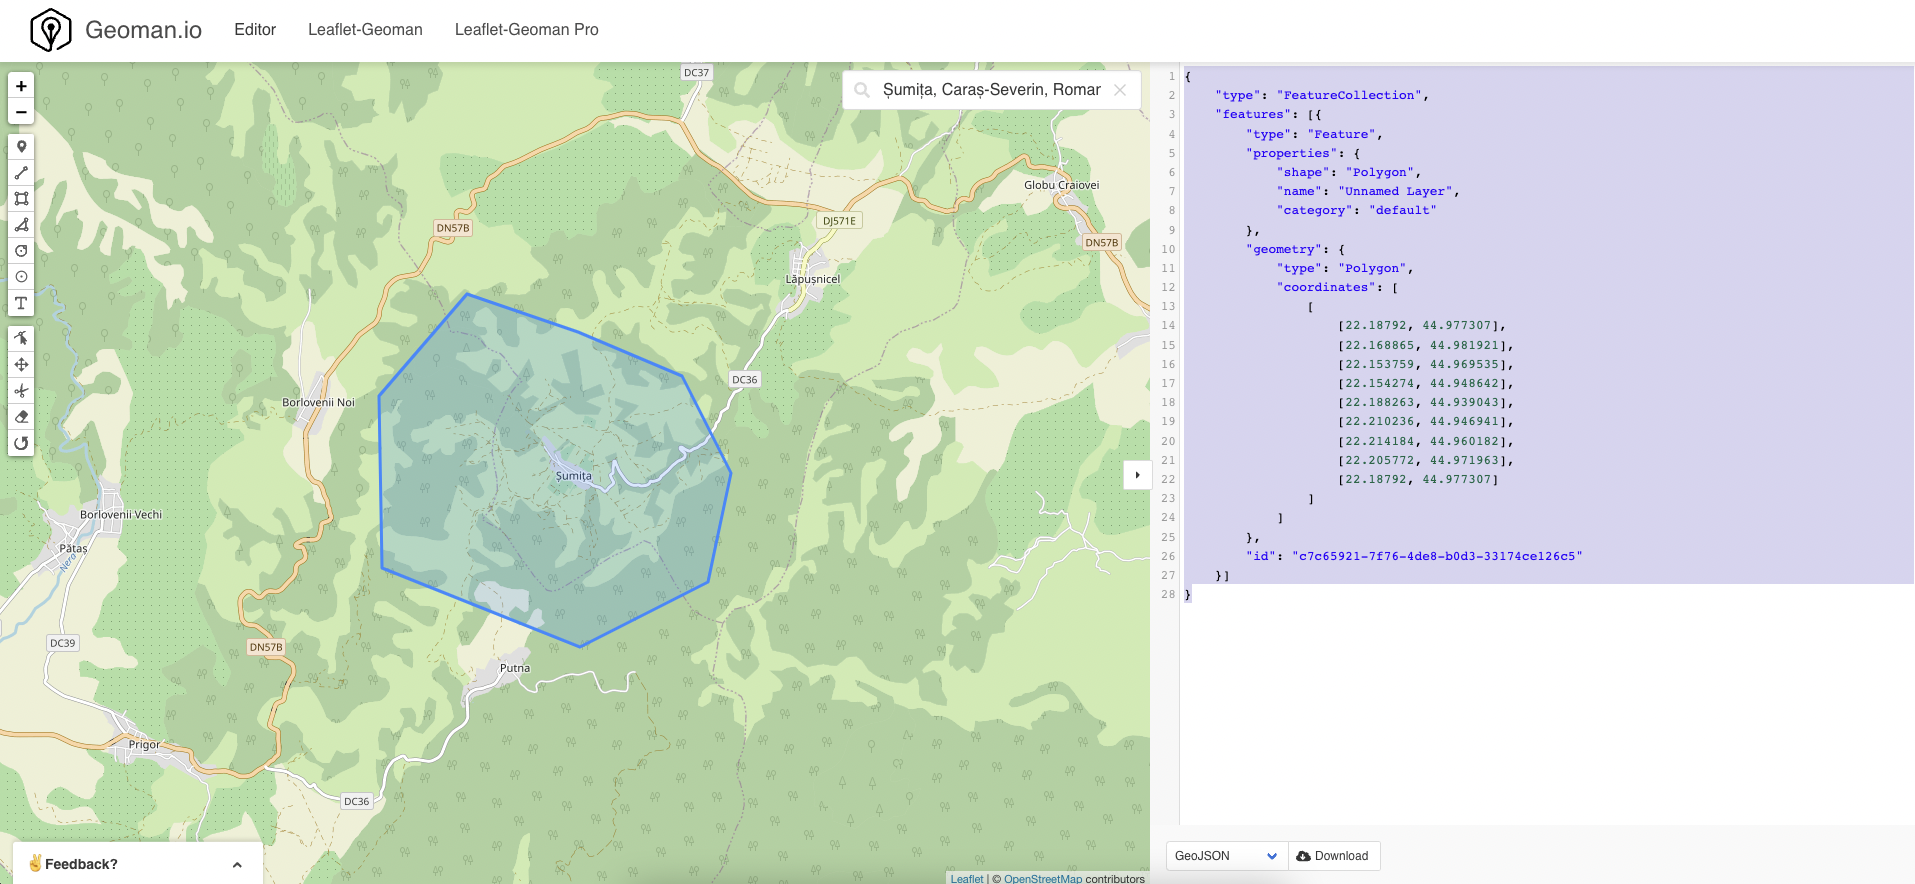
\includegraphics[width=0.95\textwidth]{geoman}  
    \caption{Rozhraní služby Geoman.io}
    \label{geoman}
\end{figure}

Závěrečnou obrazovkou, jež zmíníme, je sekce \emph{O~projektu} (viz obrázek \ref{about}). Ta je v~tuto chvíli spíše marginálnější povahy, protože obsahuje pouze základní informace o~celém projektu. Nicméně do budoucna může být prostorem pro další informace, jako jsou například nápověda nebo odkazy na přidružené projekty.

\begin{figure}
    \centering
    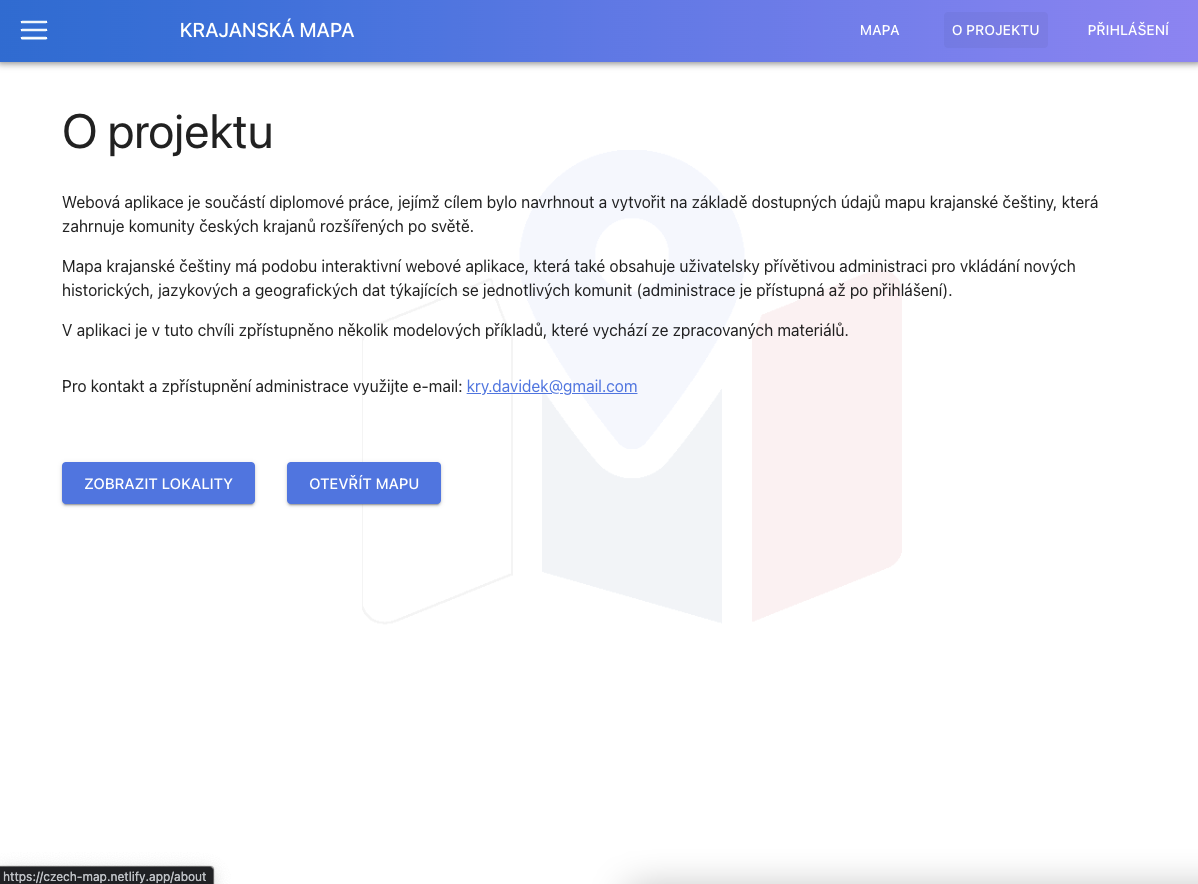
\includegraphics[width=0.95\textwidth]{about}  
    \caption{Informační stránka o~projektu}
    \label{about}
\end{figure}

\hypertarget{responzivnuxed-design}{%
\subsection{Responzivní design}\label{responzivnuxed-design}}

Jedním z~nefunkčních požadavků na aplikaci je její multiplatformní povaha. To v~praxi znamená, že by naše řešení mělo být použitelné napříč zařízeními s~různým rozlišením apod.

Jelikož jsme vyvíjeli webovou aplikaci, museli jsme tak brát ohled na zásady responzivního designu. Jedná se o~způsob stylování HTML (prostřednictvím pomocí CSS, ale i~JavaScriptu) pomocí různých flexibilních struktur, jehož výsledkem má být optimální zobrazení na všech možných obrazovkách.

Tento požadavek se nám povedlo naplnit (viz obrázky \ref{resA} a~\ref{resB}), ačkoliv u~administrace nepředpokládáme tak hojné využívání na menších zařízeních. Zároveň se u~dotykových zařízení lehce mění způsob využívání některých komponent (např. mapa nebo obrázková galerie), které jsou tak uzpůsobeny na dotykovou interakci.

\begin{figure}
    \centering
  \begin{subfigure}[b]{0.45\textwidth}
      \centering
    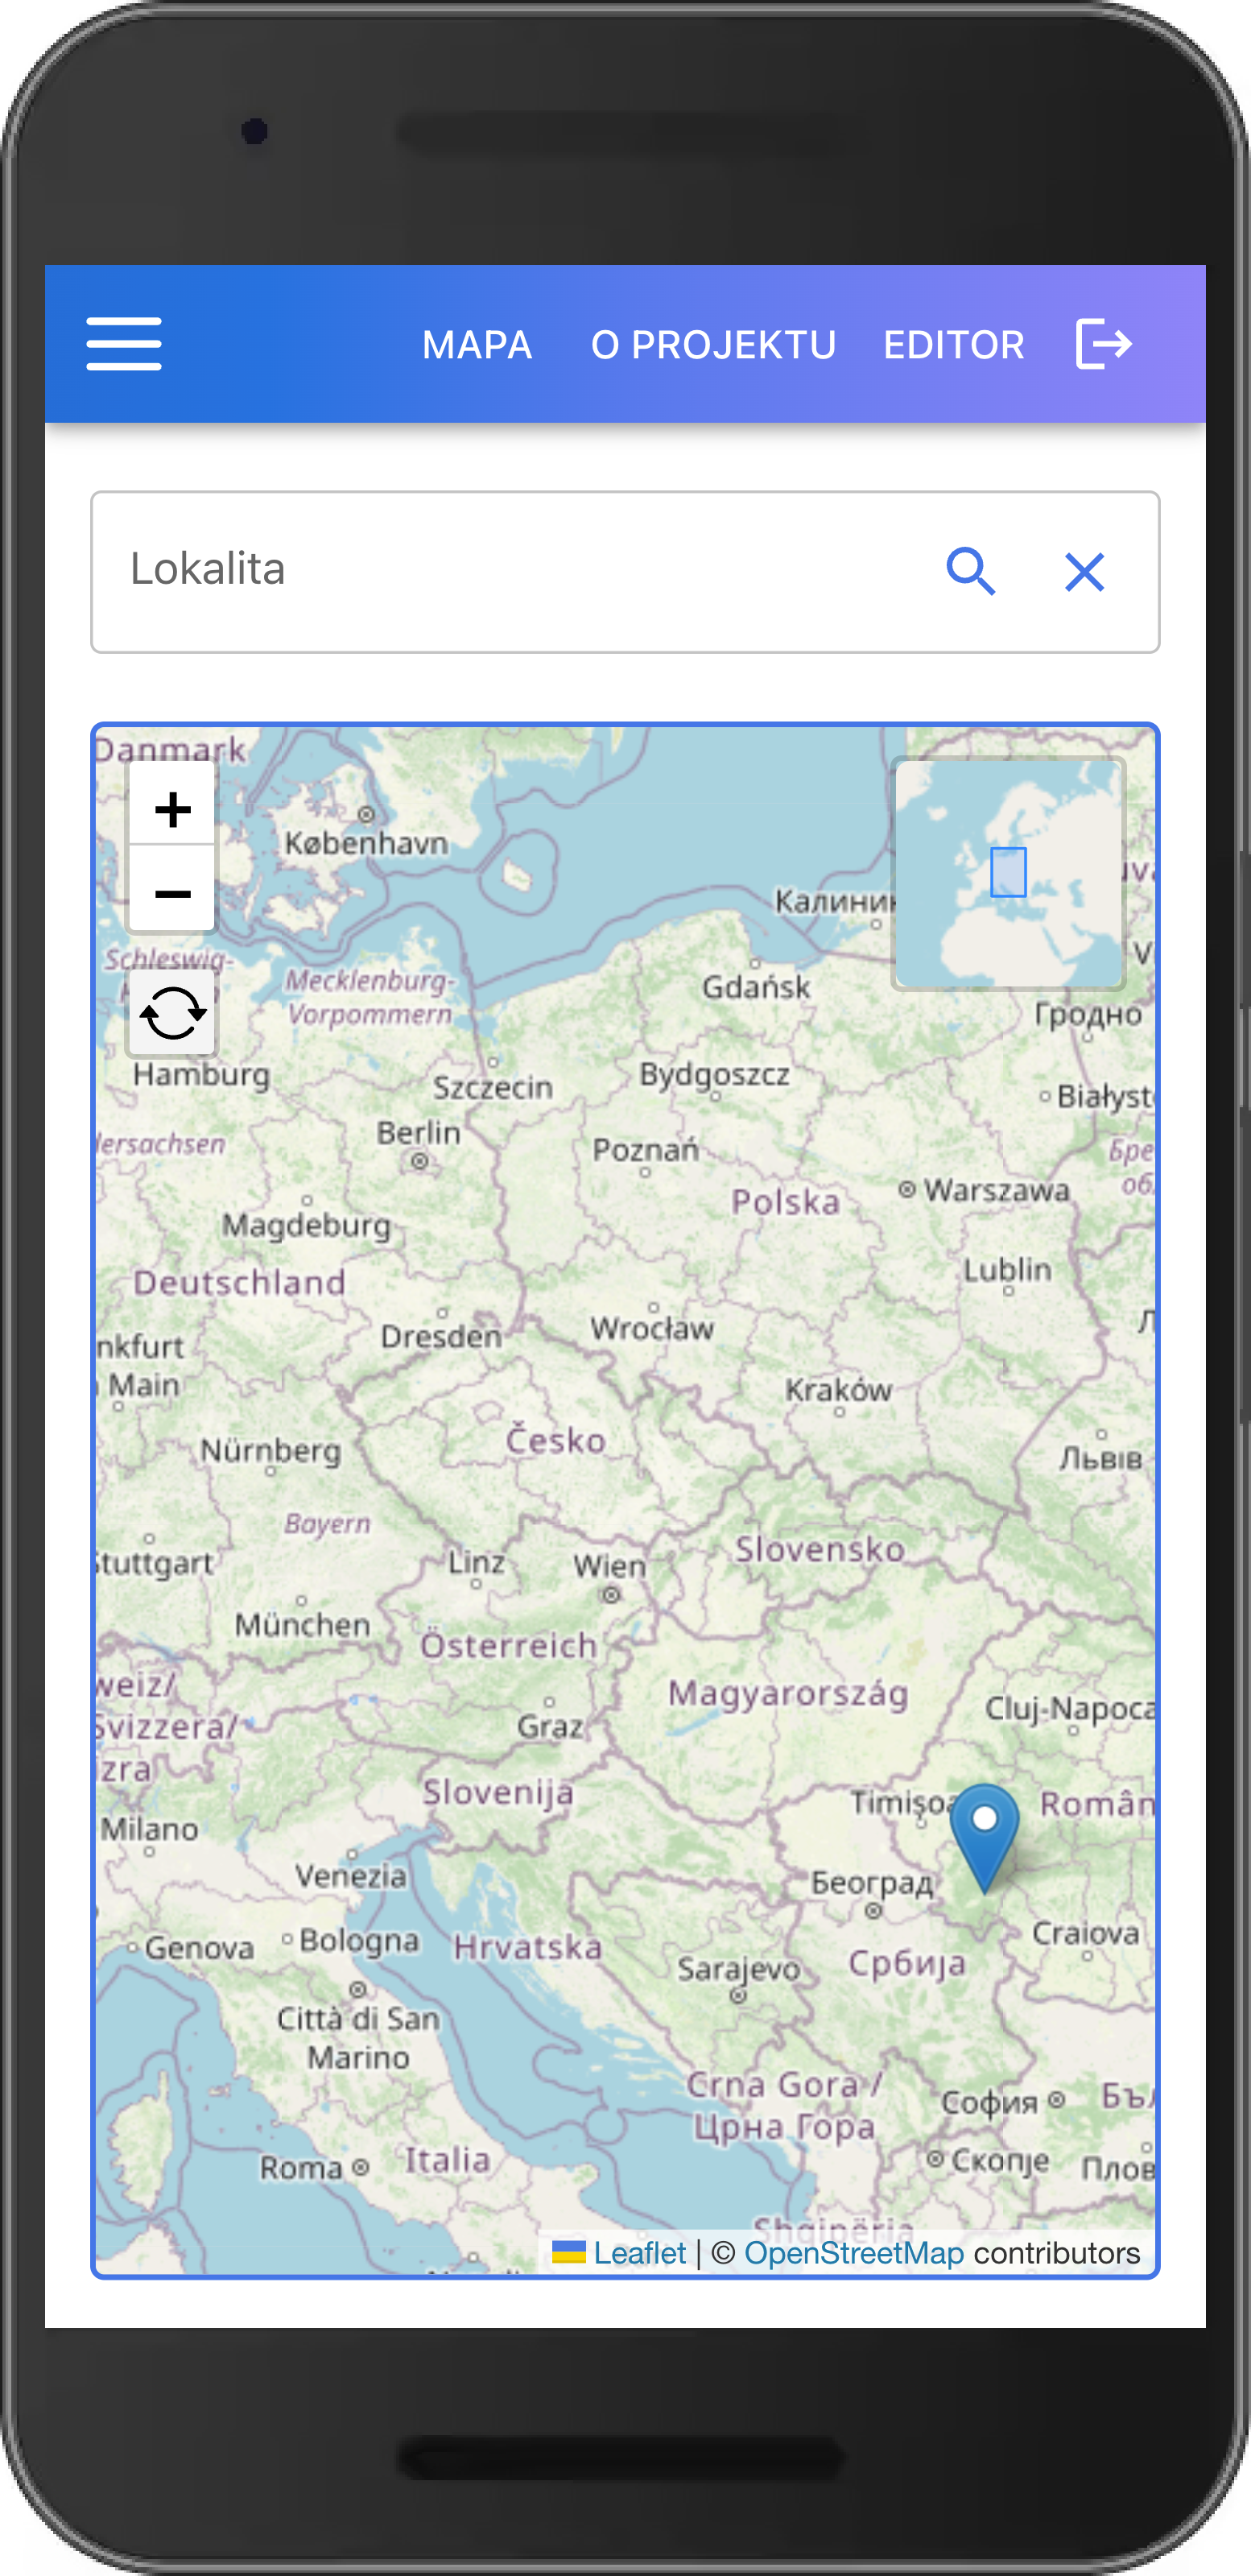
\includegraphics[width=0.7\textwidth]{res1}
  \end{subfigure}
  \hfill
  \begin{subfigure}[b]{0.45\textwidth}
      \centering
    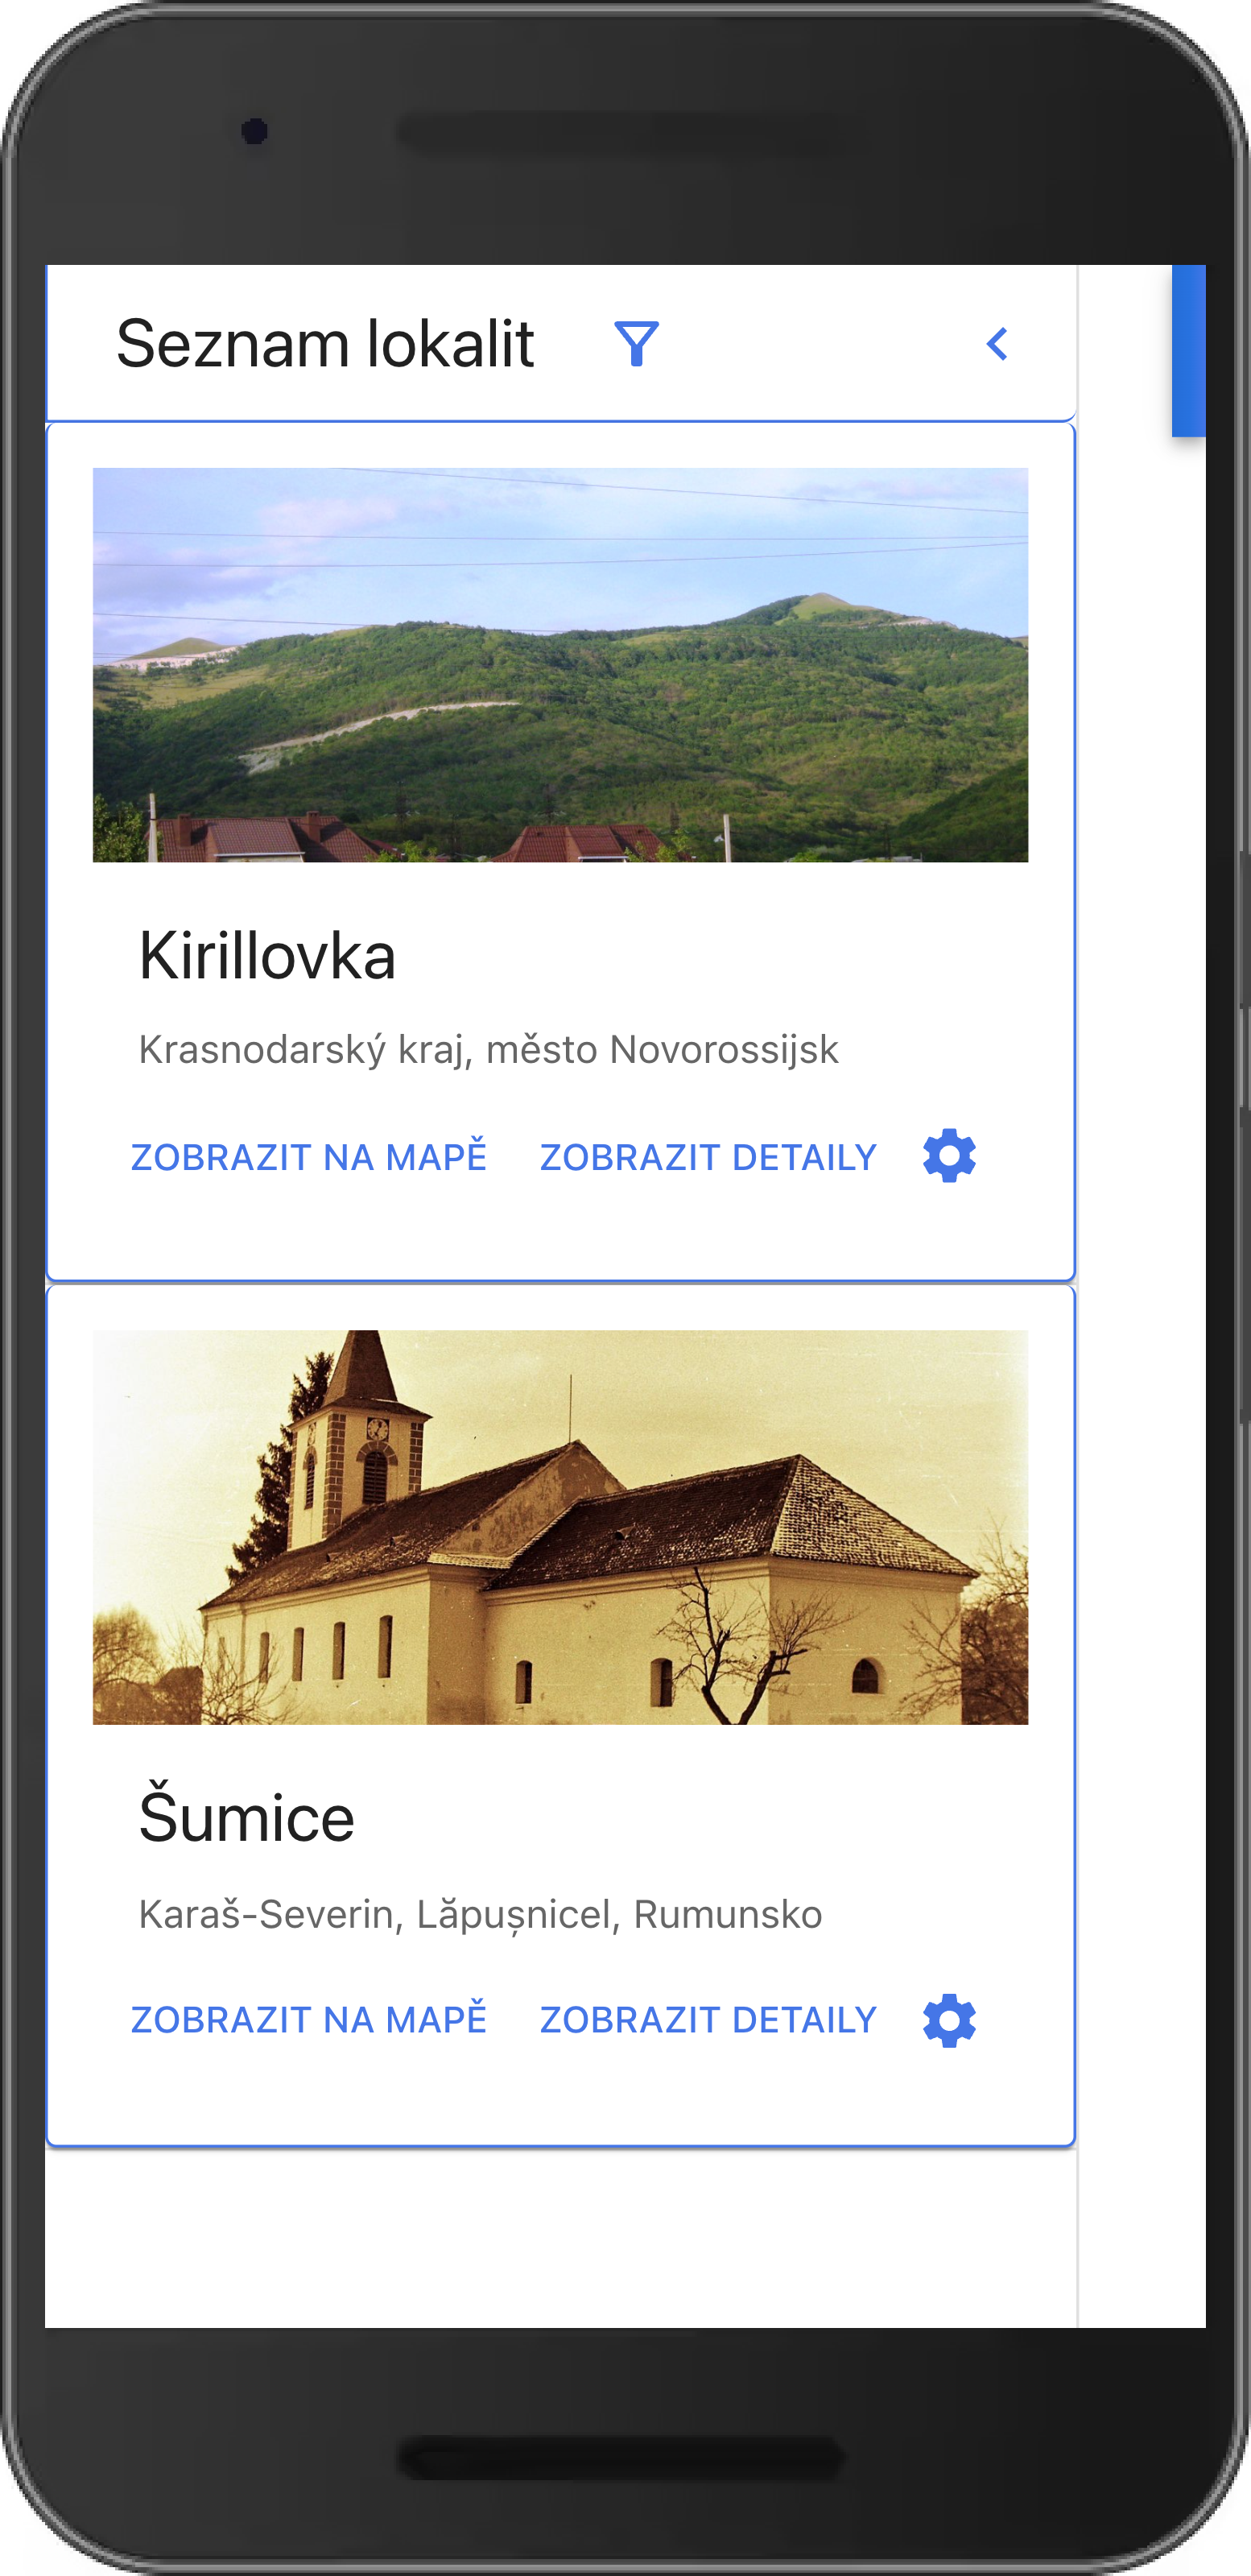
\includegraphics[width=0.7\textwidth]{res2}
  \end{subfigure}
  \caption{Responzivní zobrazení mapy a~seznamu lokalit}
  \label{resA}
\end{figure}

\begin{figure}

  \begin{subfigure}[b]{0.45\textwidth}
      \centering
    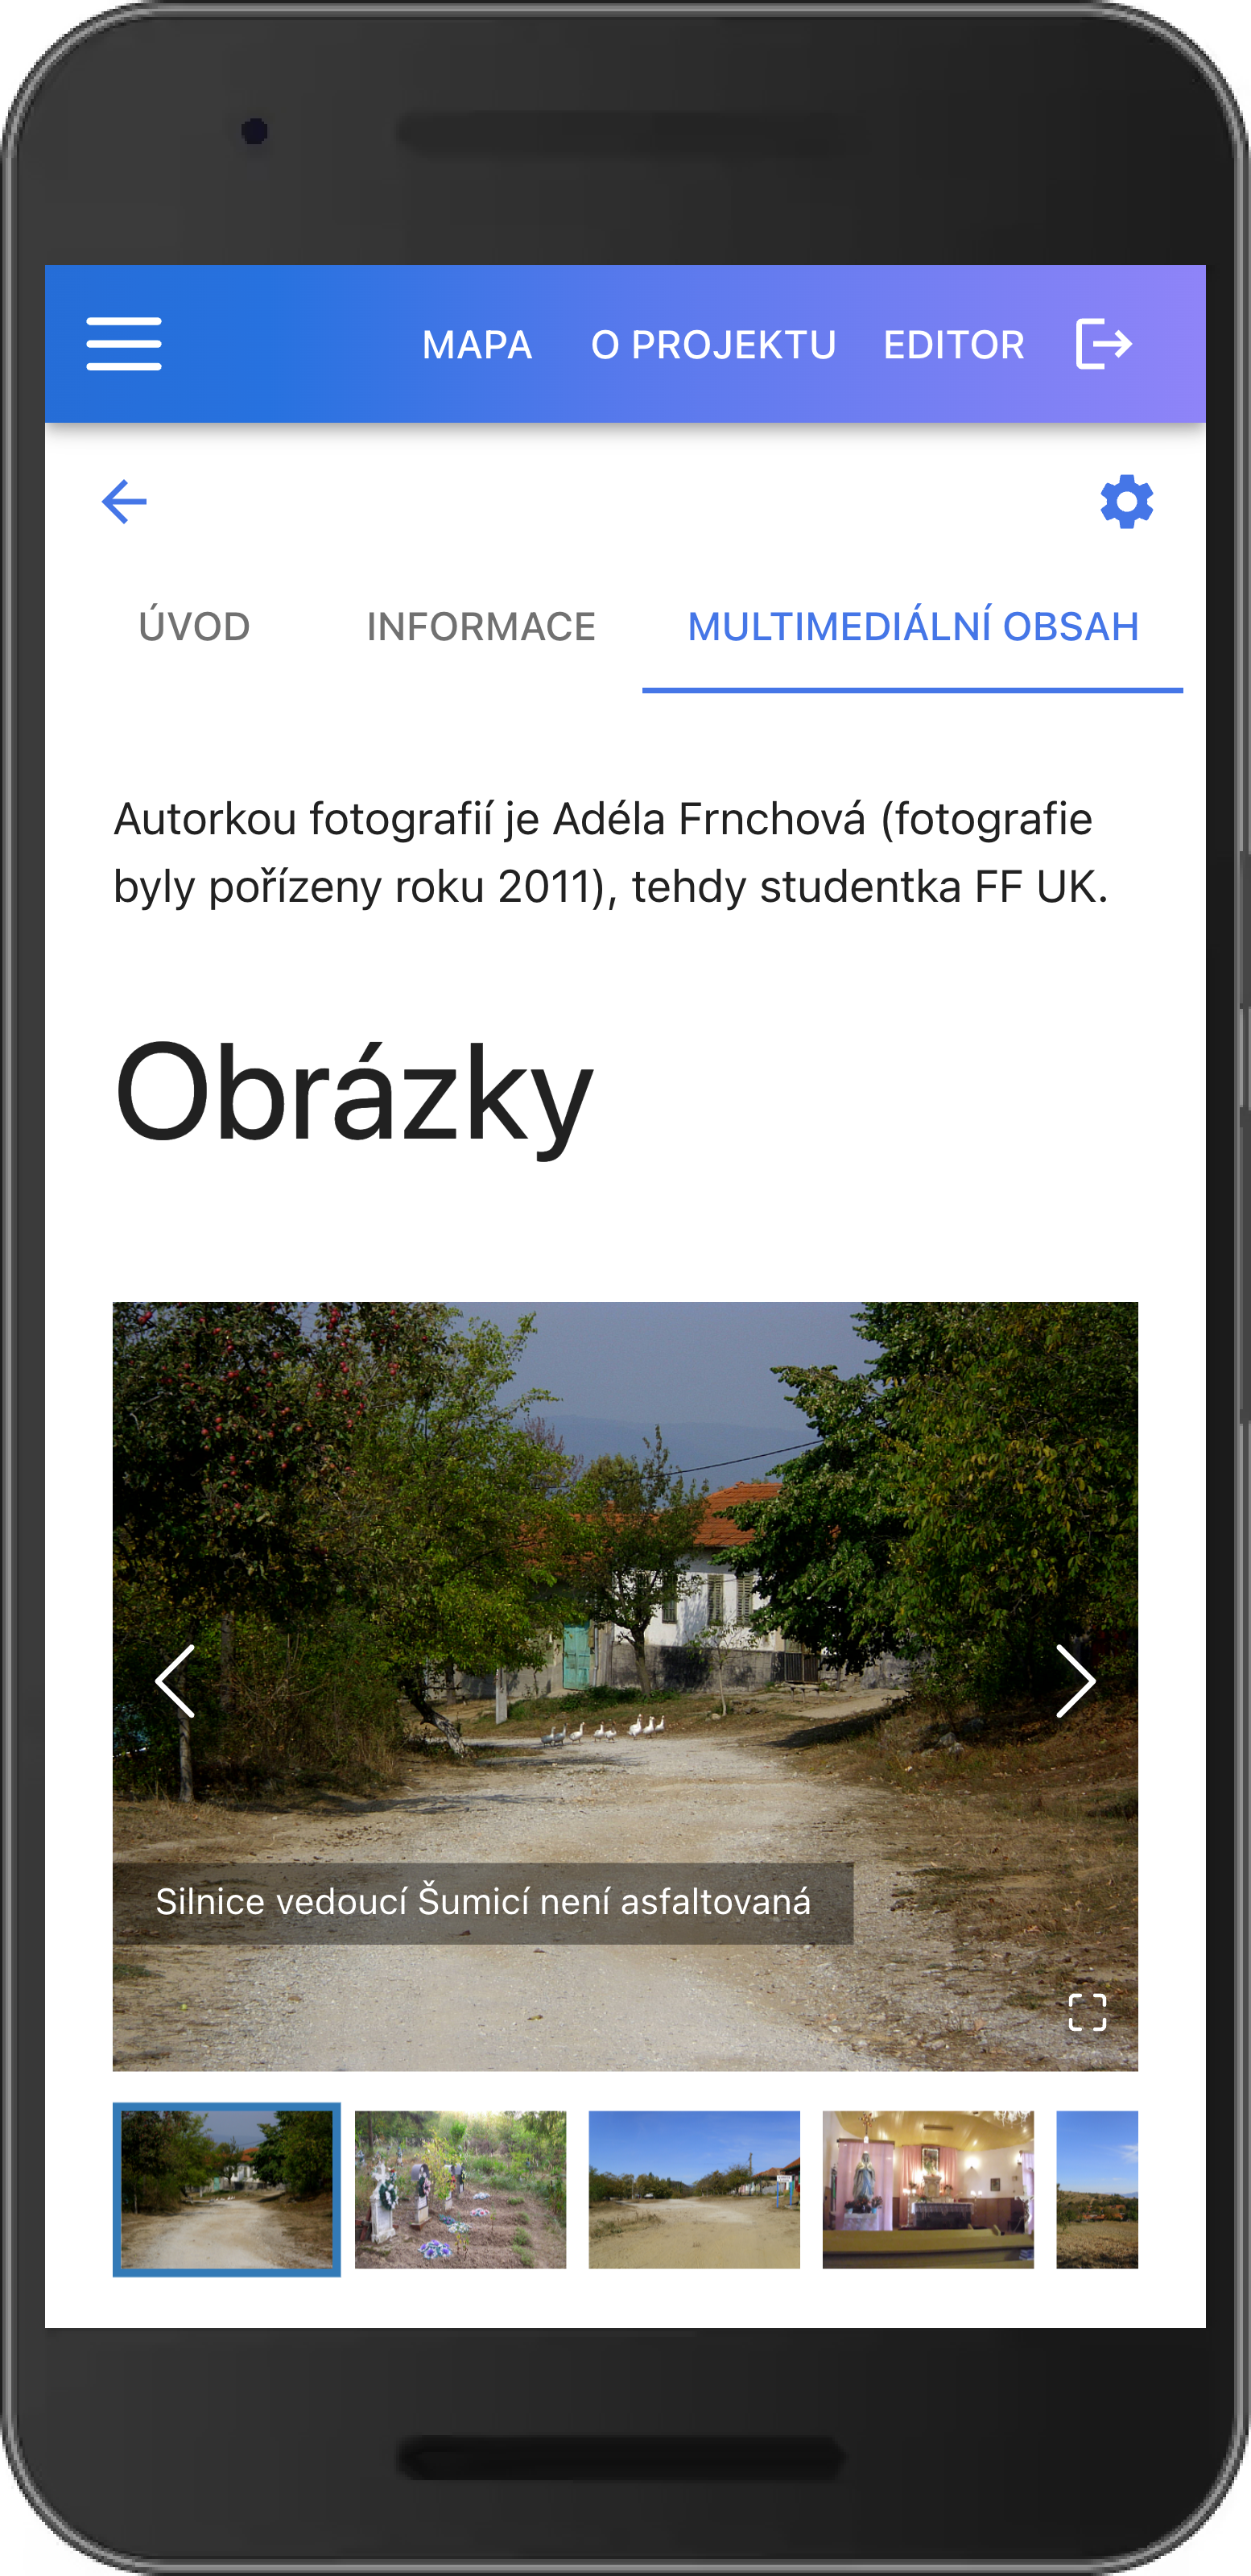
\includegraphics[width=0.7\textwidth]{res3}
  \end{subfigure}
  \hfill
  \begin{subfigure}[b]{0.45\textwidth}
      \centering
    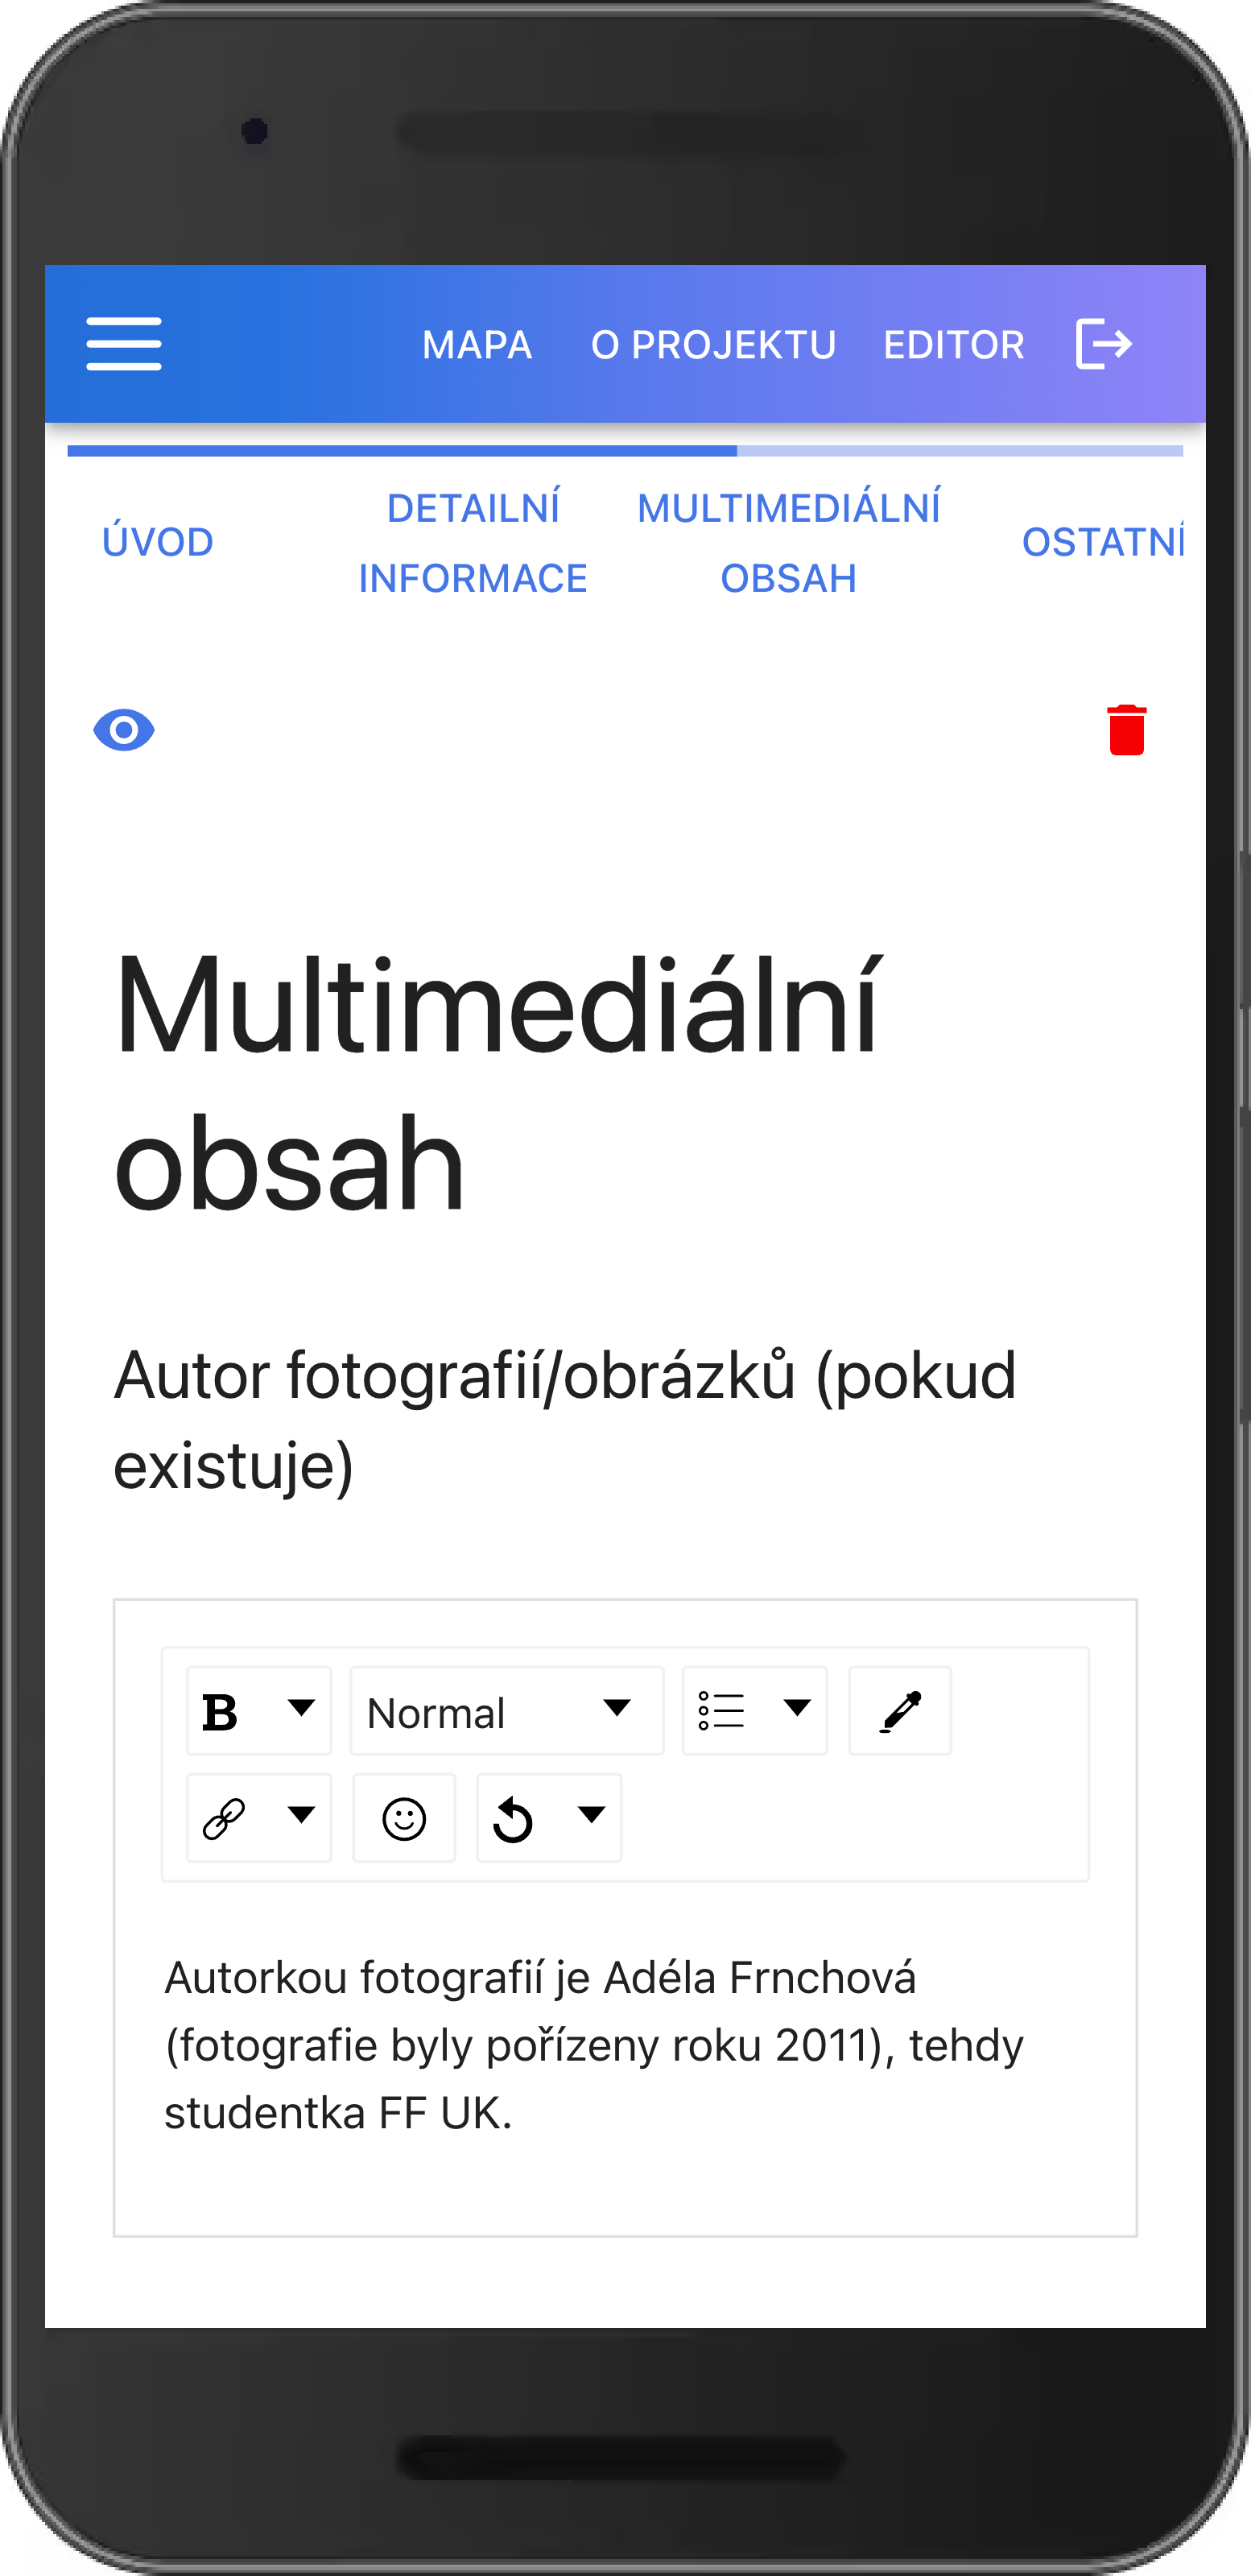
\includegraphics[width=0.7\textwidth]{res4}
  \end{subfigure}
  \caption{Responzivní zobrazení obrázkové galerie a~administrace}
  \label{resB}
\end{figure}

\hypertarget{implementace}{%
\chapter{Implementace}\label{implementace}}

V~poslední části této práce se zaměříme na implementační detaily webové aplikace. Implementaci představíme ve čtyřech částech, z~nichž se každá věnuje jiné obecnější oblasti nebo naopak konkrétní důležité funkcionalitě. V~rozsahu této práce tak není komentovat kód jako celek, ten lze však nalézt jako přílohu přiloženou k~této práci.

\hypertarget{systuxe9m-modulux16f-a-komponent}{%
\section{Systém modulů a~komponent}\label{systuxe9m-modulux16f-a-komponent}}

Jelikož je naše aplikace založena na webovém frameworku React, drželi jsme se při tvorbě všech souborů standardní adresářové struktury. Jednotlivé reactí komponenty jsou umístěny v~adresáři \verb|components|, zde je jsou tedy soubory týkající se primárně UI konkrétních částí aplikace. Zbytek komponent je pak ve složce \verb|pages|, kde jsou izolovány stránky aplikace.

\dirtree{%
.1 src.
.2 assets.
.2 components.
.3 Dialogs.
.3 Entry.
.3 Form.
.3 Map.
.2 contexts.
.2 data.
.2 hooks.
.2 models.
.2 pages.
.2 utils.
}

Při tvorbě komponent jsme se snažili o~co největší modularitu z~hlediska funkcionalit jednotlivých částí. Níže uvádíme příklad komponenty \verb|Gallery|, která obsahuje logiku a~UI pro obrázkovou galerii.

Komponentu definujeme jako javaScriptovou funkci a~za vstupní parametr (objekt \emph{props}) vkládáme danou část dostupných dat typu \verb|GalleryProps| (jde o~seznam názvů souborů a~jejich případných popisků).

Na začátku probíhá inicializace vstupních dat, jimž předchází validace a~další procedury. V~příkladu si navíc můžeme všimnout využití takzvaných \emph{hooks} (reactí funkce, které začínají slovem \emph{use}, například tedy \verb|useState|), které typicky spravují stav komponenty.

\begin{verbatim}
const Gallery = ({ dropZone }: GalleryProps) => {
    const { urls, setNames } = useAsyncFiles();
    const [loading, setLoading] = useState<boolean>(true);
    
    const [images, setImages] = useState<
        {
            original: string | undefined;
            thumbnail: string | undefined;
            description: string | undefined;
        }[]
    >([]);
    
if (!dropZone.files[0]) return  <></>;
    ...
\end{verbatim}

Jelikož je komponenta \verb|Gallery| závislá na datech z~externí databáze, musí nejprve proběhnout stáhnutí požadovaných souborů. To probíhá prostřednictvím jiného \emph{hooku} \verb|useEffect|, který se vždy spouští při změně hodnoty proměnné, která je definovaná na konci funkce v~takzvaném \emph{dependency array}. Takto si komponenta na základě vstupních dat zavolá asynchronní funkci, z~předchozí ukázky \verb|setNames| z~hooku \verb|useAsyncFiles|, která izolovaně komunikuje s~databází a~přiřazuje výsledné URL adresy souborů do proměnné \verb|urls|. Výhodou tohoto principu je nezávislost komponent na aktuálně používaném řešení pro stahování dat.

\begin{verbatim}
...
useEffect(() => {
  if (urls?.[0]) {
    const newImages = urls.map((url, i) => ({
      original: url,
      thumbnail: url,
      description: dropZone.names[i] ? .name
    }));
    setImages(newImages);
    setLoading(false);
  }
}, [urls]);

useEffect(() => {
  if (dropZone.files[0]) {
    setNames(dropZone.files);
  }
}, [dropZone]);
...
\end{verbatim}

\hypertarget{stavy-aplikace}{%
\section{Stavy aplikace}\label{stavy-aplikace}}

\hypertarget{komunikace-s-databuxe1zuxed}{%
\section{Komunikace s~databází}\label{komunikace-s-databuxe1zuxed}}

\hypertarget{mapa}{%
\section{Mapa}\label{mapa}}

\hypertarget{zuxe1vux11br}{%
\chapter*{Závěr}\label{zaver}\addcontentsline{toc}{chapter}{Závěr}}

Tohle je zaver k~diplomce

\clearpage

\pagestyle{plain}

\addcontentsline{toc}{chapter}{Seznam literatury}
\begin{spacing}{1.05}
\printbibliography[title={Seznam literatury}]
\end{spacing}

\end{document}